
%% bare_jrnl.tex
%% V1.4b
%% 2015/08/26
%% by Michael Shell
%% see http://www.michaelshell.org/
%% for current contact information.
%%
%% This is a skeleton file demonstrating the use of IEEEtran.cls
%% (requires IEEEtran.cls version 1.8b or later) with an IEEE
%% journal paper.
%%
%% Support sites:
%% http://www.michaelshell.org/tex/ieeetran/
%% http://www.ctan.org/pkg/ieeetran
%% and
%% http://www.ieee.org/

%%*************************************************************************
%% Legal Notice:
%% This code is offered as-is without any warranty either expressed or
%% implied; without even the implied warranty of MERCHANTABILITY or
%% FITNESS FOR A PARTICULAR PURPOSE! 
%% User assumes all risk.
%% In no event shall the IEEE or any contributor to this code be liable for
%% any damages or losses, including, but not limited to, incidental,
%% consequential, or any other damages, resulting from the use or misuse
%% of any information contained here.
%%
%% All comments are the opinions of their respective authors and are not
%% necessarily endorsed by the IEEE.
%%
%% This work is distributed under the LaTeX Project Public License (LPPL)
%% ( http://www.latex-project.org/ ) version 1.3, and may be freely used,
%% distributed and modified. A copy of the LPPL, version 1.3, is included
%% in the base LaTeX documentation of all distributions of LaTeX released
%% 2003/12/01 or later.
%% Retain all contribution notices and credits.
%% ** Modified files should be clearly indicated as such, including  **
%% ** renaming them and changing author support contact information. **
%%*************************************************************************


% *** Authors should verify (and, if needed, correct) their LaTeX system  ***
% *** with the testflow diagnostic prior to trusting their LaTeX platform ***
% *** with production work. The IEEE's font choices and paper sizes can   ***
% *** trigger bugs that do not appear when using other class files.       ***                          ***
% The testflow support page is at:
% http://www.michaelshell.org/tex/testflow/



\documentclass[journal]{IEEEtran}
%
% If IEEEtran.cls has not been installed into the LaTeX system files,
% manually specify the path to it like:
% \documentclass[journal]{../sty/IEEEtran}





% Some very useful LaTeX packages include:
% (uncomment the ones you want to load)


% *** MISC UTILITY PACKAGES ***
%
%\usepackage{ifpdf}
% Heiko Oberdiek's ifpdf.sty is very useful if you need conditional
% compilation based on whether the output is pdf or dvi.
% usage:
% \ifpdf
%   % pdf code
% \else
%   % dvi code
% \fi
% The latest version of ifpdf.sty can be obtained from:
% http://www.ctan.org/pkg/ifpdf
% Also, note that IEEEtran.cls V1.7 and later provides a builtin
% \ifCLASSINFOpdf conditional that works the same way.
% When switching from latex to pdflatex and vice-versa, the compiler may
% have to be run twice to clear warning/error messages.






% *** CITATION PACKAGES ***
%
%\usepackage{cite}
% cite.sty was written by Donald Arseneau
% V1.6 and later of IEEEtran pre-defines the format of the cite.sty package
% \cite{} output to follow that of the IEEE. Loading the cite package will
% result in citation numbers being automatically sorted and properly
% "compressed/ranged". e.g., [1], [9], [2], [7], [5], [6] without using
% cite.sty will become [1], [2], [5]--[7], [9] using cite.sty. cite.sty's
% \cite will automatically add leading space, if needed. Use cite.sty's
% noadjust option (cite.sty V3.8 and later) if you want to turn this off
% such as if a citation ever needs to be enclosed in parenthesis.
% cite.sty is already installed on most LaTeX systems. Be sure and use
% version 5.0 (2009-03-20) and later if using hyperref.sty.
% The latest version can be obtained at:
% http://www.ctan.org/pkg/cite
% The documentation is contained in the cite.sty file itself.






% *** GRAPHICS RELATED PACKAGES ***
%
\ifCLASSINFOpdf
 \usepackage[pdftex]{graphicx}
  % declare the path(s) where your graphic files are
  % \graphicspath{{../pdf/}{../jpeg/}}
  % and their extensions so you won't have to specify these with
  % every instance of \includegraphics
  % \DeclareGraphicsExtensions{.pdf,.jpeg,.png}
\else
  % or other class option (dvipsone, dvipdf, if not using dvips). graphicx
  % will default to the driver specified in the system graphics.cfg if no
  % driver is specified.
  % \usepackage[dvips]{graphicx}
  % declare the path(s) where your graphic files are
  % \graphicspath{{../eps/}}
  % and their extensions so you won't have to specify these with
  % every instance of \includegraphics
  % \DeclareGraphicsExtensions{.eps}
\fi
% graphicx was written by David Carlisle and Sebastian Rahtz. It is
% required if you want graphics, photos, etc. graphicx.sty is already
% installed on most LaTeX systems. The latest version and documentation
% can be obtained at: 
% http://www.ctan.org/pkg/graphicx
% Another good source of documentation is "Using Imported Graphics in
% LaTeX2e" by Keith Reckdahl which can be found at:
% http://www.ctan.org/pkg/epslatex
%
% latex, and pdflatex in dvi mode, support graphics in encapsulated
% postscript (.eps) format. pdflatex in pdf mode supports graphics
% in .pdf, .jpeg, .png and .mps (metapost) formats. Users should ensure
% that all non-photo figures use a vector format (.eps, .pdf, .mps) and
% not a bitmapped formats (.jpeg, .png). The IEEE frowns on bitmapped formats
% which can result in "jaggedy"/blurry rendering of lines and letters as
% well as large increases in file sizes.
%
% You can find documentation about the pdfTeX application at:
% http://www.tug.org/applications/pdftex





% *** MATH PACKAGES ***
%
\usepackage{amsmath}
% A popular package from the American Mathematical Society that provides
% many useful and powerful commands for dealing with mathematics.
%
% Note that the amsmath package sets \interdisplaylinepenalty to 10000
% thus preventing page breaks from occurring within multiline equations. Use:
%\interdisplaylinepenalty=2500
% after loading amsmath to restore such page breaks as IEEEtran.cls normally
% does. amsmath.sty is already installed on most LaTeX systems. The latest
% version and documentation can be obtained at:
% http://www.ctan.org/pkg/amsmath
%\usepackage{amsaddr}		
%\usepackage{amsthm}		
%\usepackage{amsaddr}		
\usepackage{amsfonts}		





% *** SPECIALIZED LIST PACKAGES ***
%
%\usepackage{algorithmic}
% algorithmic.sty was written by Peter Williams and Rogerio Brito.
% This package provides an algorithmic environment fo describing algorithms.
% You can use the algorithmic environment in-text or within a figure
% environment to provide for a floating algorithm. Do NOT use the algorithm
% floating environment provided by algorithm.sty (by the same authors) or
% algorithm2e.sty (by Christophe Fiorio) as the IEEE does not use dedicated
% algorithm float types and packages that provide these will not provide
% correct IEEE style captions. The latest version and documentation of
% algorithmic.sty can be obtained at:
% http://www.ctan.org/pkg/algorithms
% Also of interest may be the (relatively newer and more customizable)
% algorithmicx.sty package by Szasz Janos:
% http://www.ctan.org/pkg/algorithmicx




% *** ALIGNMENT PACKAGES ***
%
%\usepackage{array}
% Frank Mittelbach's and David Carlisle's array.sty patches and improves
% the standard LaTeX2e array and tabular environments to provide better
% appearance and additional user controls. As the default LaTeX2e table
% generation code is lacking to the point of almost being broken with
% respect to the quality of the end results, all users are strongly
% advised to use an enhanced (at the very least that provided by array.sty)
% set of table tools. array.sty is already installed on most systems. The
% latest version and documentation can be obtained at:
% http://www.ctan.org/pkg/array


% IEEEtran contains the IEEEeqnarray family of commands that can be used to
% generate multiline equations as well as matrices, tables, etc., of high
% quality.




% *** SUBFIGURE PACKAGES ***
%\ifCLASSOPTIONcompsoc
%  \usepackage[caption=false,font=normalsize,labelfont=sf,textfont=sf]{subfig}
%\else
%  \usepackage[caption=false,font=footnotesize]{subfig}
%\fi
% subfig.sty, written by Steven Douglas Cochran, is the modern replacement
% for subfigure.sty, the latter of which is no longer maintained and is
% incompatible with some LaTeX packages including fixltx2e. However,
% subfig.sty requires and automatically loads Axel Sommerfeldt's caption.sty
% which will override IEEEtran.cls' handling of captions and this will result
% in non-IEEE style figure/table captions. To prevent this problem, be sure
% and invoke subfig.sty's "caption=false" package option (available since
% subfig.sty version 1.3, 2005/06/28) as this is will preserve IEEEtran.cls
% handling of captions.
% Note that the Computer Society format requires a larger sans serif font
% than the serif footnote size font used in traditional IEEE formatting
% and thus the need to invoke different subfig.sty package options depending
% on whether compsoc mode has been enabled.
%
% The latest version and documentation of subfig.sty can be obtained at:
% http://www.ctan.org/pkg/subfig




% *** FLOAT PACKAGES ***
%
%\usepackage{fixltx2e}
% fixltx2e, the successor to the earlier fix2col.sty, was written by
% Frank Mittelbach and David Carlisle. This package corrects a few problems
% in the LaTeX2e kernel, the most notable of which is that in current
% LaTeX2e releases, the ordering of single and double column floats is not
% guaranteed to be preserved. Thus, an unpatched LaTeX2e can allow a
% single column figure to be placed prior to an earlier double column
% figure.
% Be aware that LaTeX2e kernels dated 2015 and later have fixltx2e.sty's
% corrections already built into the system in which case a warning will
% be issued if an attempt is made to load fixltx2e.sty as it is no longer
% needed.
% The latest version and documentation can be found at:
% http://www.ctan.org/pkg/fixltx2e


%\usepackage{stfloats}
% stfloats.sty was written by Sigitas Tolusis. This package gives LaTeX2e
% the ability to do double column floats at the bottom of the page as well
% as the top. (e.g., "\begin{figure*}[!b]" is not normally possible in
% LaTeX2e). It also provides a command:
%\fnbelowfloat
% to enable the placement of footnotes below bottom floats (the standard
% LaTeX2e kernel puts them above bottom floats). This is an invasive package
% which rewrites many portions of the LaTeX2e float routines. It may not work
% with other packages that modify the LaTeX2e float routines. The latest
% version and documentation can be obtained at:
% http://www.ctan.org/pkg/stfloats
% Do not use the stfloats baselinefloat ability as the IEEE does not allow
% \baselineskip to stretch. Authors submitting work to the IEEE should note
% that the IEEE rarely uses double column equations and that authors should try
% to avoid such use. Do not be tempted to use the cuted.sty or midfloat.sty
% packages (also by Sigitas Tolusis) as the IEEE does not format its papers in
% such ways.
% Do not attempt to use stfloats with fixltx2e as they are incompatible.
% Instead, use Morten Hogholm'a dblfloatfix which combines the features
% of both fixltx2e and stfloats:
%
% \usepackage{dblfloatfix}
% The latest version can be found at:
% http://www.ctan.org/pkg/dblfloatfix




%\ifCLASSOPTIONcaptionsoff
%  \usepackage[nomarkers]{endfloat}
% \let\MYoriglatexcaption\caption
% \renewcommand{\caption}[2][\relax]{\MYoriglatexcaption[#2]{#2}}
%\fi
% endfloat.sty was written by James Darrell McCauley, Jeff Goldberg and 
% Axel Sommerfeldt. This package may be useful when used in conjunction with 
% IEEEtran.cls'  captionsoff option. Some IEEE journals/societies require that
% submissions have lists of figures/tables at the end of the paper and that
% figures/tables without any captions are placed on a page by themselves at
% the end of the document. If needed, the draftcls IEEEtran class option or
% \CLASSINPUTbaselinestretch interface can be used to increase the line
% spacing as well. Be sure and use the nomarkers option of endfloat to
% prevent endfloat from "marking" where the figures would have been placed
% in the text. The two hack lines of code above are a slight modification of
% that suggested by in the endfloat docs (section 8.4.1) to ensure that
% the full captions always appear in the list of figures/tables - even if
% the user used the short optional argument of \caption[]{}.
% IEEE papers do not typically make use of \caption[]'s optional argument,
% so this should not be an issue. A similar trick can be used to disable
% captions of packages such as subfig.sty that lack options to turn off
% the subcaptions:
% For subfig.sty:
% \let\MYorigsubfloat\subfloat
% \renewcommand{\subfloat}[2][\relax]{\MYorigsubfloat[]{#2}}
% However, the above trick will not work if both optional arguments of
% the \subfloat command are used. Furthermore, there needs to be a
% description of each subfigure *somewhere* and endfloat does not add
% subfigure captions to its list of figures. Thus, the best approach is to
% avoid the use of subfigure captions (many IEEE journals avoid them anyway)
% and instead reference/explain all the subfigures within the main caption.
% The latest version of endfloat.sty and its documentation can obtained at:
% http://www.ctan.org/pkg/endfloat
%
% The IEEEtran \ifCLASSOPTIONcaptionsoff conditional can also be used
% later in the document, say, to conditionally put the References on a 
% page by themselves.




% *** PDF, URL AND HYPERLINK PACKAGES ***
%
%\usepackage{url}
% url.sty was written by Donald Arseneau. It provides better support for
% handling and breaking URLs. url.sty is already installed on most LaTeX
% systems. The latest version and documentation can be obtained at:
% http://www.ctan.org/pkg/url
% Basically, \url{my_url_here}.


%DEFS. RODNEY%%%%%%%%%%%%%%%%%%%%%%%%%%%%%%%%%%%%%
\def\bSig\mathbf{\Sigma}
\newcommand{\VS}{V\&S}
\usepackage{url}
\usepackage{soul} % allows to pass a line in words
\newcommand{\Z}{\mathbb{Z}} % Set of integers
\newcommand{\re}{\mathbb{R}} % Set of real numbers
\newcommand{\sgn}{\mathrm{sign}} % Signal operador
\newcommand{\ci}{\mathrm{i}}
\def\sT{\mbox{\tiny$T$}}
\def\E{\mbox{{\rm E\,}}}
\def\cov{\mbox{{\rm cov\,}}}
\def\corr{\mbox{{\rm corr\,}}}
\def\var{\mbox{{\rm var\,}}}
\newcommand{\vgamma}{\pmb{\gamma}}
\newcommand{\vrho}{\pmb{\rho}}
\newcommand{\vbeta}{\pmb{\beta}}
\newcommand{\vepsilon}{\pmb{\epsilon}}
\newcommand{\vxi}{\pmb{\xi}}
\def\shalf{\mbox{{\tiny$\frac{1}{2}$}}}
\def\half{\mbox{{\small$\frac{1}{2}$}}}
%\newtheorem{theorem}{Theorem}{\bf}{\rm}  
\newtheorem{lemma}{Lemma}

\newcommand{\vA}{{\textbf A}}
\newcommand{\vD}{{\textbf D}}
\newcommand{\vd}{{\textbf d}}
\newcommand{\vW}{{\textbf W}}
\newcommand{\vR}{{\textbf R}}
\newcommand{\vS}{{\textbf S}}
\newcommand{\vU}{{\textbf U}}
\newcommand{\vI}{{\textbf I}}
\newcommand{\vX}{{\textbf X}}
\newcommand{\vf}{{\textbf f}}
\newcommand{\vu}{{\textbf u}}
\newcommand{\vT}{{\textbf T}}
\newcommand{\vt}{{\textbf t}}
\newcommand{\vy}{{\textbf y}}


\usepackage{hyperref}

%DEFS. ROGERIO%%%%%%%%%%%%%%%%%%%%%%%%%%%%%%%%%%%%
%\usepackage{graphicx}

\usepackage{subfigure}
\usepackage{multirow}
\usepackage{color,colortbl}
\usepackage{enumerate}
\usepackage{amsmath,amssymb}
\usepackage{booktabs}
\usepackage{rotating}
\usepackage{cite}
\usepackage{balance}

\usepackage{bm,bbm}
\usepackage{datetime2}
\usepackage[binary-units]{siunitx}

\usepackage{mathrsfs}

\usepackage{placeins}

\usepackage[abs]{overpic}
\usepackage{pict2e}
%\usepackage{float}
\usepackage{microtype}
\usepackage{pdfpages}

\makeatletter
\newcommand{\thickhline}{\noalign {\ifnum 0=`}\fi \hrule height 1pt \futurelet \reserved@a \@xhline}
\newcolumntype{"}{@{\hskip\tabcolsep\vrule width 1pt\hskip\tabcolsep}}
\makeatother
%%%%%%%%%%%%%%%%%%%%%%%%%%%%%%%%%%%%%%%%%%%%%%%%%%

% *** Do not adjust lengths that control margins, column widths, etc. ***
% *** Do not use packages that alter fonts (such as pslatex).         ***
% There should be no need to do such things with IEEEtran.cls V1.6 and later.
% (Unless specifically asked to do so by the journal or conference you plan
% to submit to, of course. )


% correct bad hyphenation here
\hyphenation{op-tical net-works semi-conduc-tor}


\begin{document}
%
% paper title
% Titles are generally capitalized except for words such as a, an, and, as,
% at, but, by, for, in, nor, of, on, or, the, to and up, which are usually
% not capitalized unless they are the first or last word of the title.
% Linebreaks \\ can be used within to get better formatting as desired.
% Do not put math or special symbols in the title.
\title{Wavelet Spatio-Temporal Change Detection on multi-temporal SAR images}
%
%
% author names and IEEE memberships
% note positions of commas and nonbreaking spaces ( ~ ) LaTeX will not break
% a structure at a ~ so this keeps an author's name from being broken across
% two lines.
% use \thanks{} to gain access to the first footnote area
% a separate \thanks must be used for each paragraph as LaTeX2e's \thanks
% was not built to handle multiple paragraphs
%

\author{Rodney~V.~Fonseca, Rog\'{e}rio~G.~Negri,
        Alu\'{i}sio~Pinheiro,
        and~Abdourrahmane~Atto,~\IEEEmembership{Senior~Member,~IEEE}% <-this % stops a space
\thanks{This work was supported by FAPESP grants 2016/24469-6 and 2018/04654-9 and CNPq grants 309230/2017-9 and 310991/2020-0.}
\thanks{R.~Fonseca and A.~Pinheiro are with the Department of Statistics, University of Campinas, Campinas 13083-859, Brazil (e-mails: ra192588@dac.unicamp.br; pinheiro@ime.unicamp.br).}
\thanks{A.~Atto is with the LISTIC - Polytech Annecy-Chamb\'{e}ry, Universit\'{e} de Savoie, 74944 Annecy le Vieux Cedex, France (e-mail: Abdourrahmane.Atto@univ-savoie.fr).}
\thanks{R.~G.~Negri is with the Department of Environmental Engineering, São Paulo State University, São José dos Campos, Brazil (e-mail: rogerio.negri@unesp.br).}
}
% <-this % stops a space
%\thanks{Manuscript received April 19, 2005; revised August 26, 2015.}}

% note the % following the last \IEEEmembership and also \thanks - 
% these prevent an unwanted space from occurring between the last author name
% and the end of the author line. i.e., if you had this:
% 
% \author{....lastname \thanks{...} \thanks{...} }
%                     ^------------^------------^----Do not want these spaces!
%
% a space would be appended to the last name and could cause every name on that
% line to be shifted left slightly. This is one of those "LaTeX things". For
% instance, "\textbf{A} \textbf{B}" will typeset as "A B" not "AB". To get
% "AB" then you have to do: "\textbf{A}\textbf{B}"
% \thanks is no different in this regard, so shield the last } of each \thanks
% that ends a line with a % and do not let a space in before the next \thanks.
% Spaces after \IEEEmembership other than the last one are OK (and needed) as
% you are supposed to have spaces between the names. For what it is worth,
% this is a minor point as most people would not even notice if the said evil
% space somehow managed to creep in.



% The paper headers
\markboth{Journal of \LaTeX\ Class Files,~Vol.~X, No.~X, Month~20XX}%
{Shell \MakeLowercase{\textit{et al.}}: Bare Demo of IEEEtran.cls for IEEE Journals}
% The only time the second header will appear is for the odd numbered pages
% after the title page when using the twoside option.
% 
% *** Note that you probably will NOT want to include the author's ***
% *** name in the headers of peer review papers.                   ***
% You can use \ifCLASSOPTIONpeerreview for conditional compilation here if
% you desire.




% If you want to put a publisher's ID mark on the page you can do it like
% this:
%\IEEEpubid{0000--0000/00\$00.00~\copyright~2015 IEEE}
% Remember, if you use this you must call \IEEEpubidadjcol in the second
% column for its text to clear the IEEEpubid mark.



% use for special paper notices
%\IEEEspecialpapernotice{(Invited Paper)}




% make the title area
\maketitle

% As a general rule, do not put math, special symbols or citations
% in the abstract or keywords.
\begin{abstract}
We introduce WECS (Wavelet Energies Correlation Screening), an unsupervised procedure to detect spatio-temporal change points on multi-temporal SAR images. The procedure is based on wavelet approximation for the multi-temporal images, wavelet energy apportionment, and ultra-high dimensional correlation screening for the wavelet coefficients. We show WECS performance on simulated multi-temporal image data. We also evaluate the proposed method on a time series of 84 satellite images in a forest region at the border of Brazil and the French Guiana. The proposed method displays good results in covering change regions, with the additional benefit of having simple and fast computation.
\end{abstract}

% Note that keywords are not normally used for peerreview papers.
\begin{IEEEkeywords}
Change detection, Remote Sensing, multi-temporal images, simulated images, wavelets.
\end{IEEEkeywords}






% For peer review papers, you can put extra information on the cover
% page as needed:
% \ifCLASSOPTIONpeerreview
% \begin{center} \bfseries EDICS Category: 3-BBND \end{center}
% \fi
%
% For peerreview papers, this IEEEtran command inserts a page break and
% creates the second title. It will be ignored for other modes.
\IEEEpeerreviewmaketitle



\section{Introduction}
% The very first letter is a 2 line initial drop letter followed
% by the rest of the first word in caps.
% 
% form to use if the first word consists of a single letter:
% \IEEEPARstart{A}{demo} file is ....
% 
% form to use if you need the single drop letter followed by
% normal text (unknown if ever used by the IEEE):
% \IEEEPARstart{A}{}demo file is ....
% 
% Some journals put the first two words in caps:
% \IEEEPARstart{T}{his demo} file is ....
% 
% Here we have the typical use of a "T" for an initial drop letter
% and "HIS" in caps to complete the first word.

\IEEEPARstart{C}{hange} detection is an important task performed in remote sensing image that allows researchers and engineers to identify and evaluate modifications on land surfaces captured by multi-temporal satellite images. Analyzing problems such as deforestation \cite{barreto2016deforestation}, rapid urbanization \cite{ban2012multitemporal} and glacier melting \cite{scher2021mapping} are of great importance to study the dynamics of regions sensitive to climate changes and human activity. Furthermore, the increase on availability of satellite images in the past years raises the challenge of applying computationally cheap methods to images available at larger and larger from time to time. A review for change detection in multi-temporal remote sensing is given by \cite{ban2016change}.


Most methods used for change detection analysis can be classified either as supervised (training data is used to set up the method) or unsupervised (fully data-driven techniques). We shall focus in this work on unsupervised approaches, whose examples in the literature include the works of \cite{bruzzone2000automatic,celik2010change,quin2014mimosa,saha2020change,NegriEA2021,NegriFrery2021}. Many other proposals of methods vary in their motivations as well as in their applicability.  Change detection in multi-temporal hyperspectral images is discussed in \cite{bovolo2015time,liu2019review,matsunaga2017current}.  \cite{jia2018novel} pursue change detection techniques via non-local means and principal component analysis. Compressed projection and image fusion are employed by \cite{hou2014unsupervised}. Deep learning by slow feature analysis for change detection is the subject of \cite{du2019unsupervised}. \cite{chen2020change} proposes a change detection method driven by adaptive parameter estimation.

A special attention has been given for multi-temporal change detection using Synthetic Aperture Radar (SAR) images. \textcolor{green}{Some of the references already mentioned are examples of change detection methods applied to SAR images \cite{barreto2016deforestation,ban2012multitemporal,scher2021mapping,quin2014mimosa}, \cite{jia2018novel}, \cite{hou2014unsupervised}, \cite{bovolo2005detail} }. 
Known to be not affected by weather, cloud and sunlight conditions, SAR images rise as an essential data source in change detection applications \cite{bovolo2005detail}.
Conversely, due to its acquisition architecture, the speckle noise typically affects the images obtained by SAR sensors and demands additional pre-processing before its use.

Face with the complexity imposed by the high-dimensionality of multi-temporal datasets in addition to the presence of speckle noise, the change detection process using SAR images becomes a challenge task.
In this context, the use of Wavelets rises as a convenient approach once such technique is robust when dealing with noise data and is allows an efficient computational treatment. 

In more details, Wavelet methods present many advantages for a plethora of statistical applications \cite{vidakovic1999statistical} not only in remote sensing problems thanks to wavelet capabilities in capturing multi-scale/resolution information. 
Their computational efficiency and sparseness are specially relevant for large images and other high-dimensional data \cite{morettin2017wavelets}. 
Analysis of SAR images have been investigated under different approaches using wavelet methods, such as \cite{atto2012multidate}, \cite{bouhlel2015multivariate}, \cite{celik2009multiscale}, \cite{cui2012statistical}. 
\textcolor{magenta}{However, an application of screening ideas on wavelet coefficients is still a novel approach in change detection literature, and we show it has an interesting potential to provide good results even with simple algorithms.}


In the light of presented discussions and motivations, using Wavelet and data screening concepts, we propose the Wavelet Energies Correlation Screening (WECS), a novel unsupervised multi-temporal change detection method for SAR images.
%
The main idea behind WECS is built on ultra-high dimensional feature screening for the wavelet coefficients \cite{fan2020statistical}. Such method is usually employed in high-dimensional regression models to reduce the problem's dimension by subsetting the available covariates in such a way that true covariates are among the chosen ones with high probability \cite{fan2008sure}. We show that by applying the feature screening idea on multi-temporal images, we obtain a fast and accurate method to cover change regions with good detection rates.


\textcolor{blue}{This paper is organized as follows:
% rest of the text goes as follows. 
Section \ref{section_method} introduces the problem and presents the proposed method. We show WECS performance on simulated multi-temporal image data in Section \ref{section_validation}. In Section \ref{section_realdata} we apply the proposed method to a time series of 85 satellite images in the border region of Brazil and the French Guiana, for  images captured from November 08, 2015 to December 09 2017.  Section \ref{section_discussion} concludes the paper with a discussion.}


%%%%%%%%%%%%%%%%%%%%%%%%%%%%%%%%%%%%%%%%%%
\section{Basic Theory Background}\label{section_theroy}

Wavelet methods have been widely applied to analyze images in signal processing literature, specially for tasks such as signal denoising and compression \cite{mallat1998wavelet}. The most common way of describing wavelet representations is as a multi-resolution decomposition, where a signal is represented on approximation and detail coefficients, which provide coarse and finer details of the signal, respectively. In practice, the discrete wavelet transform of matrices (image) consists in applying low and high-pass convolution filters to its rows and columns \cite{mallat1989theory}. In case of smoothing, applying such low-pass filter $J$ times to rows and columns of a matrix $\mathcal{I}$, yields a smooth image $\vX$. The number $J$ is also called resolution level, a tuning parameter for wavelet smoothing. This wavelet smoothing is employed in the next section as a denoising step for image analysis.

\textcolor{green}{
Using wavelet smoothing on the images consists in an initial step to analyze the data, but the main goal in the analysis is to find changes in space and at instants of time. The smoothed images still contain a large number of coefficients that need to be evaluated, what characterizes a high-dimensional problem with multiple time series corresponding to each location in space. Since most part of a region is usually not relevant for overall changes, we need to employ a method that retains the most important locations driving these modifications across time. Methods like variable selection are largely employed in statistics to identify the most important covariates in a study, and one method particularly efficient in identifying relevant variables is the feature screening technique.
}

Feature screening procedure is a method originally designed for ultra-high dimensional regression models \cite{fan2008sure}. In order to explain how it works, consider the usual linear regression framework where $\vy$ is a $n\times 1$ vector of observations from a response variable and $\{\vW_1 \cdots \vW_p\}$ is a $n\times p$ matrix with explanatory variables on its columns, which are used in a linear model $\vy = \sum_{i=1}^{p}\beta_i\vW_i + \vepsilon$, where $\beta_1,\ldots,\beta_p$ are unknown parameters and $\vepsilon$ is a zero mean random noise. The problem setup is that $p$ is much larger than $n$, what makes standard regression methods unfeasible, but only a handful of the available covariates are relevant for the model, i.e., have a nonzero corresponding parameter $\beta_i$. The feature screening idea consists in computing the sample correlation $\mathrm{corr}(\vy,\vW_i)$ among response and explanatory variables, and then selecting those covariates whose correlation are among the highest values. Under suitable conditions, such method is known to select a set containing all true covariates with high probability. In the image change detection problem, our idea is that a similar approach could be used to detect change locations by taking an overall change measure as response variable and local (pixel) measures as potential covariates.



%%%%%%%%%%%%%%%%%%%%%%%%%%%%%%%%%%%%%%%%%%
\section{Wavelet Energy Correlation Screening}\label{section_method}


Figure~\ref{figDiagram} depicts a high-level conceptualization for the proposed method. The elements included in such representation are formalized in the constructions as follows.


%-------------------------
\begin{figure}[htb!]
\centering
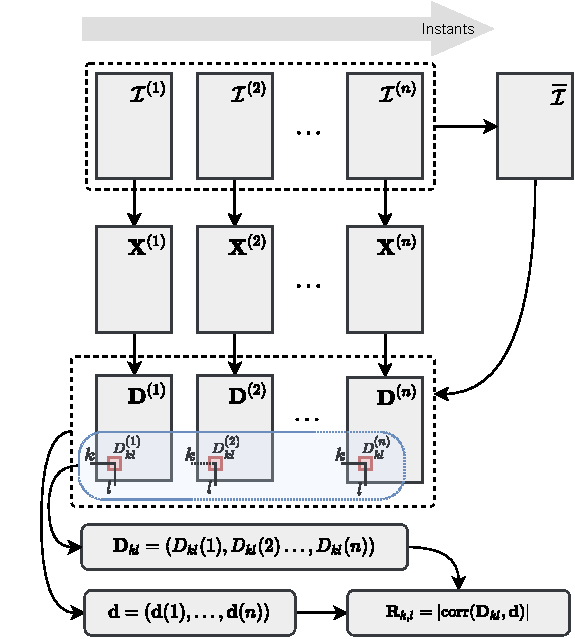
\includegraphics[scale=.8]{../../drawio/diagram_wecs.drawio_11nov21}
\caption{Diagram of steps performed on WECS to compute an absolute correlation of a single point.}
\label{figDiagram}
\end{figure}




Let $\mathcal{I}^{(1)},\ldots,\mathcal{I}^{(n)}$ be an image time series defined on a support $\mathcal{S} = \left\lbrace 1,\ldots,u  \right\rbrace \times \left\lbrace 1,\ldots,v  \right\rbrace \subset \mathbbm{N}^2$, hence representing a region of interest over $n$ distinct instants.
%
\textcolor{blue}{These images may be relative to one SAR channel or a combination of channels; this will be specified when appropriate}. Our goal is twofold: to find possible points in time where some relevant changes might have taken place at the region represented in $\mathcal{I}^{(m)}$, $m=1,\ldots,n$, and to find which regions are closely associated to the observed changes along time. We shall address these tasks by analyzing the bidimensional stationary discrete wavelet decomposition of $\mathcal{I}^{(m)}$. Stationary wavelets (also known as non-decimated or redundant wavelets) is a traditional de-noising method that can be efficiently applied to two-dimensional signals such as images \cite{coifman1995translation,atto2012multidate,atto2016wavelet}. 


After application of this wavelet transform to $\mathcal{I}^{(m)}$ at some appropriate resolution level $J\geq 1$, one of its by-products is a matrix of so called approximation wavelet coefficients $\vX^{(m)}$, a smoothed version of $\mathcal{I}^{(m)}$ 
defined on the same support $\mathcal{S}$. The higher $J\in\{1,\ldots,\log_2( \min{u,v} )\}$ is, the smoother $\vX^{(m)}$ gets.

Beyond many other aspects that can be involved in wavelet analysis of images, which may include different types of wavelet transform and basis as well the use of thresholding for detail coefficients, the current construction is focused on $\vX^{(m)}$ to provide a simple wavelet smoothing. Nevertheless, extensions based on distinct aspects are straightforward.

We can then consider further apportioning the total $\mathbb{L}_2$ energy of the series $\left\{\vX^{(m)}\right\}_{m=1,\ldots,n}$ as:
\begin{equation}\label{E:eq_ANOVAlogimage}
\begin{split}
\sum_{m=1}^n\|\vX^{(m)}\|_F^2
= n\|\overline{\mathcal{I}}\|_F^2 + 2n\langle\overline{\vX}-\overline{\mathcal{I}},\overline{\mathcal{I}}\rangle_F + \\
+ \sum_{m=1}^n\|\mathcal \vX^{(m)} - \overline{\mathcal{I}}\|_F^2,
\end{split}
\end{equation}
where $\overline{\mathcal{I}}=n^{-1}\sum_{m=1}^n\mathcal{I}^{(m)}$ and $\overline{\vX}=n^{-1}\sum_{m=1}^n\vX^{(m)}$; $\| \cdot \|_F$ and $\left\langle \cdot , \cdot \right\rangle_F$ represents the Frobenius norm and inner product, respectively. Naturally, both $\overline{\mathcal{I}}$ and $\overline{\vX}$ share the support $\mathcal{S}$.


The most right-hand term in Equation~(\ref{E:eq_ANOVAlogimage}) measures the deviations 
between the wavelet coefficients at distinct instants ($\vX^{(m)}; \ m=1,\ldots,n$) regarding the \textit{average image} (i.e., $\overline{\mathcal{I}}$). Such deviations may favor detecting relevant changes over the time. Since each element (i.e., a pixel/position $(k,l)\in \mathcal{S}$) of $\vX^{(m)}$ also has a corresponding sequence of deviations in time, the local deviation to the overall measure 
may also allow detecting the spatial changes. Among several approaches able to detect change events, the Pearson correlation coefficient rises as an convenient alternative. Furthermore, such measure \textcolor{blue}{shares connections with the idea of feature screening employed in high-dimensional regression, as explained earlier.}

Let $X_{kl}^{(m)}$ and $\overline{\mathcal{I}}_{kl}$ be the entry $(k,l)$ of $\vX^{(m)}$ and $\overline{\mathcal{I}}$, respectively. 
%
The matrix $\vD^{(m)}$ embraces the squared differences between $\vX^{(m)}$ and $\overline{\mathcal{I}}$, where $D_{kl}^{(m)} = \left( \vX_{kl}^{m} - \overline{\mathcal{I}}_{kl} \right)^2$.
%
Therefore, it is defined the temporal overall variation sequence $\left\lbrace \vd^{(m)}  \right\rbrace_{m=1,\ldots,n}$, whose elements are given by:
\begin{equation}\label{E:eq_defdm}
\vd(m)= \sum_{k=1}^{u} \sum_{l=1}^{v} D_{kl}^{(m)} %; \ m=1,\ldots,n
\end{equation}


In this context, an instant $m$ in $\left\lbrace \vd^{(m)}  \right\rbrace_{m=1,\ldots,n}$ with high value stands for the image $\mathcal{I}^{(m)}$ where the most expressive changes take place.



In order to identify spatio-temporal changes, we employ the concept of ultra-high dimensional correlation screening \cite{fan2020statistical} discussed in Section~\ref{section_theroy}. For each local squared deviation time series given by individual elements of $\vD^{(m)}$ across $m=1,\ldots,n$, \textcolor{blue}{say $\vD_{kl} = \left\lbrace D_{kl}^{(1)},\ldots,D_{kl}^{(n)} \right\rbrace$}, consider the absolute value of its Pearson correlation with the overall squared deviations, given by $\vd$:
\begin{equation*}\label{def_Rkld}
R_{kl}= |\corr \left( \vD_{kl}, \vd \right)|.
\end{equation*}
Consequently, rises the matrix $\vR$ from the elements $R_{kl}$ assigned to each $(k,l) \in \mathcal{S}$.




Let us define a mapping of \textit{important} indices for changes over the image series with respect to $\overline{\mathcal I}$ as $\mathcal{M}^{\star} \subseteq \mathcal{S}$ where \textit{changes in $\{\mathcal{I}^{(m)}\}_{m=1,\ldots,n}$ with respect to $\overline{\mathcal{I}}$ are affected by local changes in the images}.




An empirical mapping of change locations may be stated by:
\begin{equation}
\mathcal{M}_{\tau} = \{(k,l) \in \mathcal{S} : |R_{kl}|>\tau\},
\label{E:def_Mtaud}
\end{equation}
where $\tau \in \mathbbm{R}_{+}^{*}$ is a convenient threshold value. Under \textcolor{green}{some regularity conditions \cite{fan2020statistical}}, the probability $P(\mathcal{M}_{\tau}\supset\mathcal{M}^{\star}) \rightarrow 1$ as $n\rightarrow\infty$. In other words, the empirical set $\mathcal{M}_{\tau}$ has high probability of detecting the correct change locations in $\mathcal{M}^{\star}$ when the number of instants $n$ is large enough. 




\section{Experiments}

In this section we shall evaluate the performance of WECS on two types of data sets. Initially, we generate simulated data where the level of noise and true change regions are known. For these images, we analyze different aspects of concerning the application of WECS and compare its performance with a standard change detection method. In the following application, real satellite data is employed, where the performance of WECS is evaluated on predefined change regions.

\subsection{Simulated data analysis}\label{secExpSimulated}

In this section we apply the change detection methods above on simulated data of multi-temporal images. The simulated multi-temporal images ($n=80$) is obtained by repeating a sequence of four images with different types of changes plus a noise. Examples of the first four of these images are shown in Figure \ref{F:EllipsoidChanges}. These images are generated from the sum of two matrices: a signal matrix with ones on entries where ellipses occur and zero elsewhere, and a noise matrix with random variables following a standard Gaussian distribution. The first image, $\mathcal{I}^{(1)}$, presents three elongated ellipses. The second image $\mathcal{I}^{(2)}$ has shorter and larger ellipses added. Smaller ellipses are then added to form $\mathcal{I}^{(3)}$ and $\mathcal{I}^{(4)}$. All the changes made that occur among subsequent images can be seen in Figure \ref{F:Changes_methods_images}(a), which displays a matrix of zeros and ones that correspond, respectively, to locations without and with changes along time. Applying WECS to these images, we obtain a matrix $\vR$ of correlations between deviations of each $\mathcal{I}$ entry with the total squared mean deviation. An example of $\vR$ is presented in Figure \ref{F:Changes_methods_images}(b). For some choice of threshold $\tau$ on absolute values of $\vR$, we obtain a matrix of zeros and ones that can be compared with the total true changes displayed in Figure \ref{F:Changes_methods_images}(a).

\begin{figure}[htb!]
\centering
%\includegraphics[width=40pc]{EllipsoidChanges/ellipses_all}
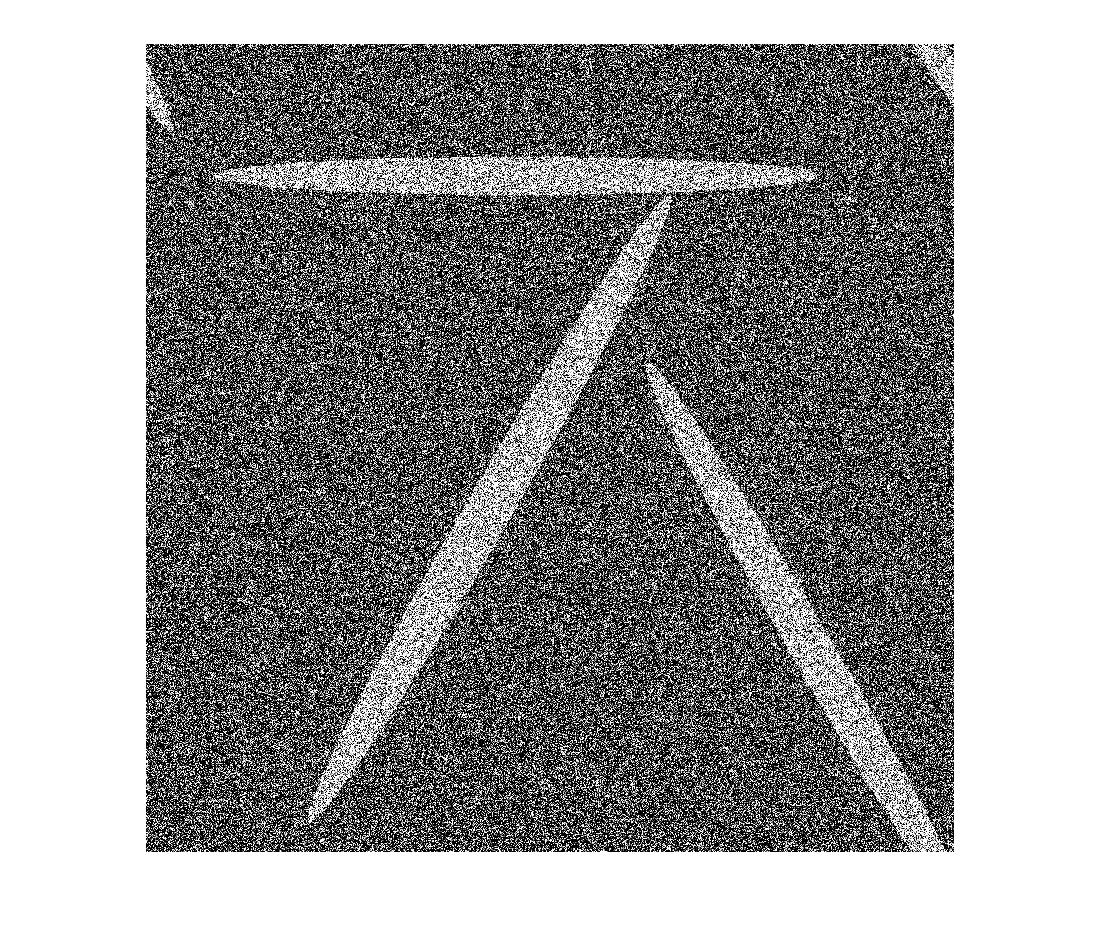
\includegraphics[scale=.11]{../../figs/ellipses_t1}
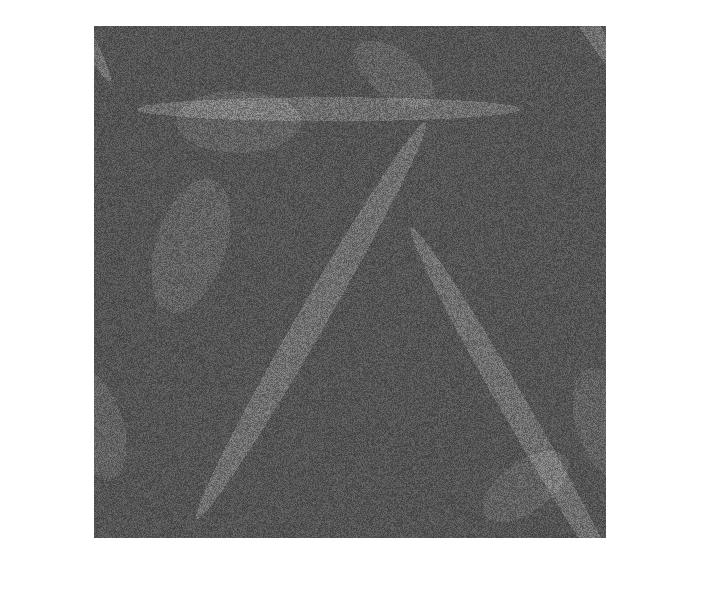
\includegraphics[scale=.11]{../../figs/ellipses_t2}
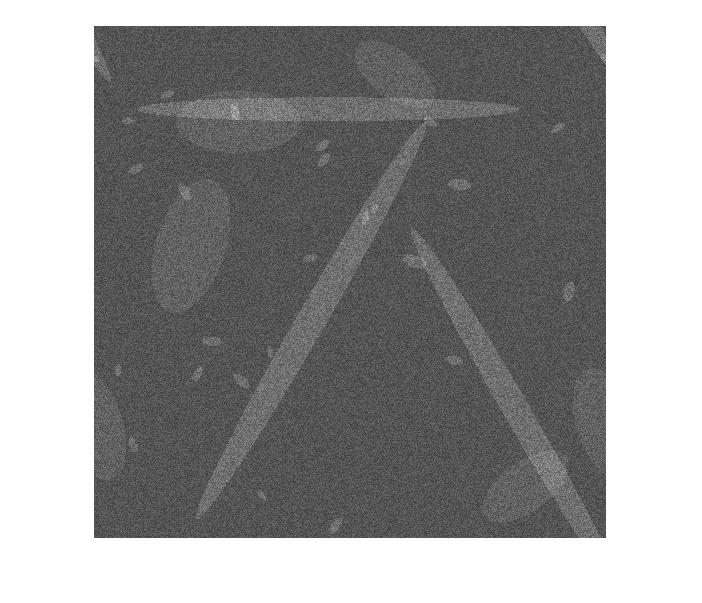
\includegraphics[scale=.11]{../../figs/ellipses_t3}
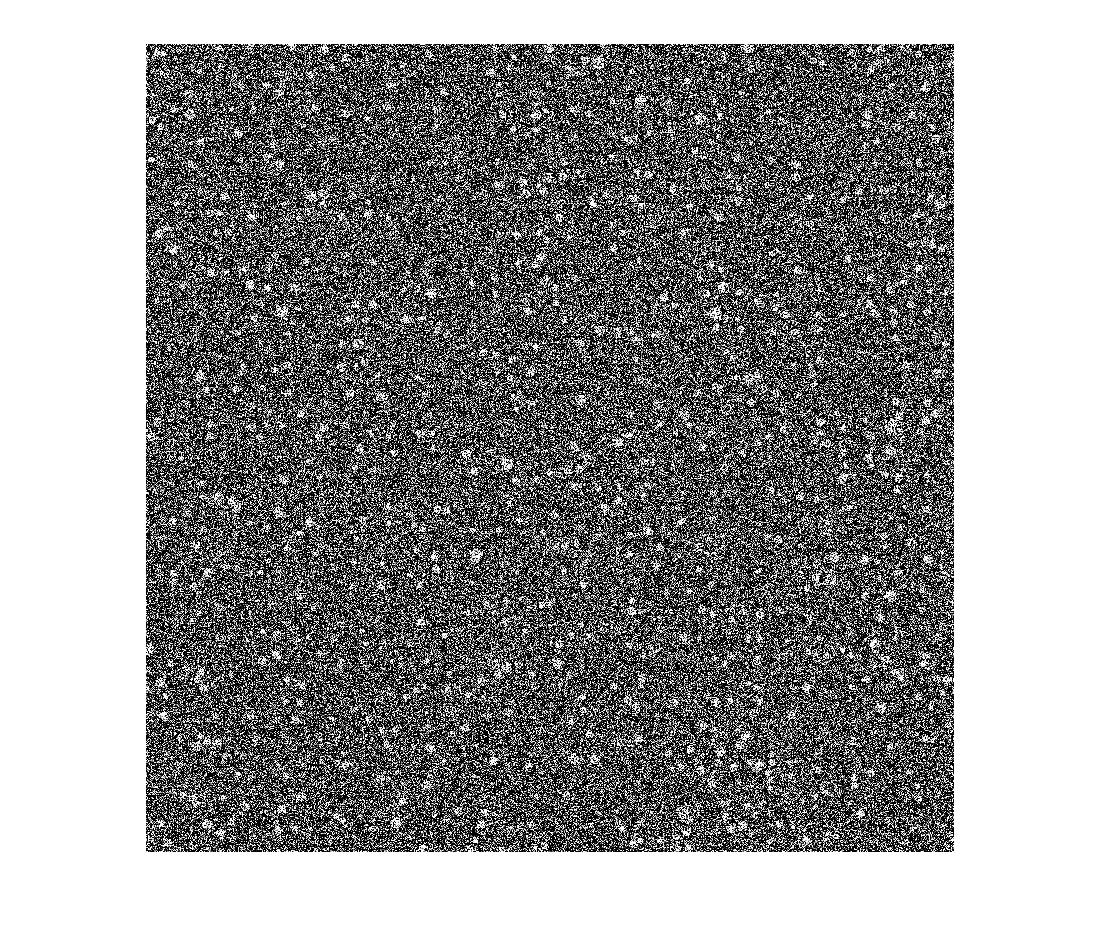
\includegraphics[scale=.11]{../../figs/ellipses_t4}
\caption{Example of the first four simulated multi-temporal images. Features and changes come as white ellipses and dots.}
\label{F:EllipsoidChanges}
\end{figure}


\begin{figure}[htp!]
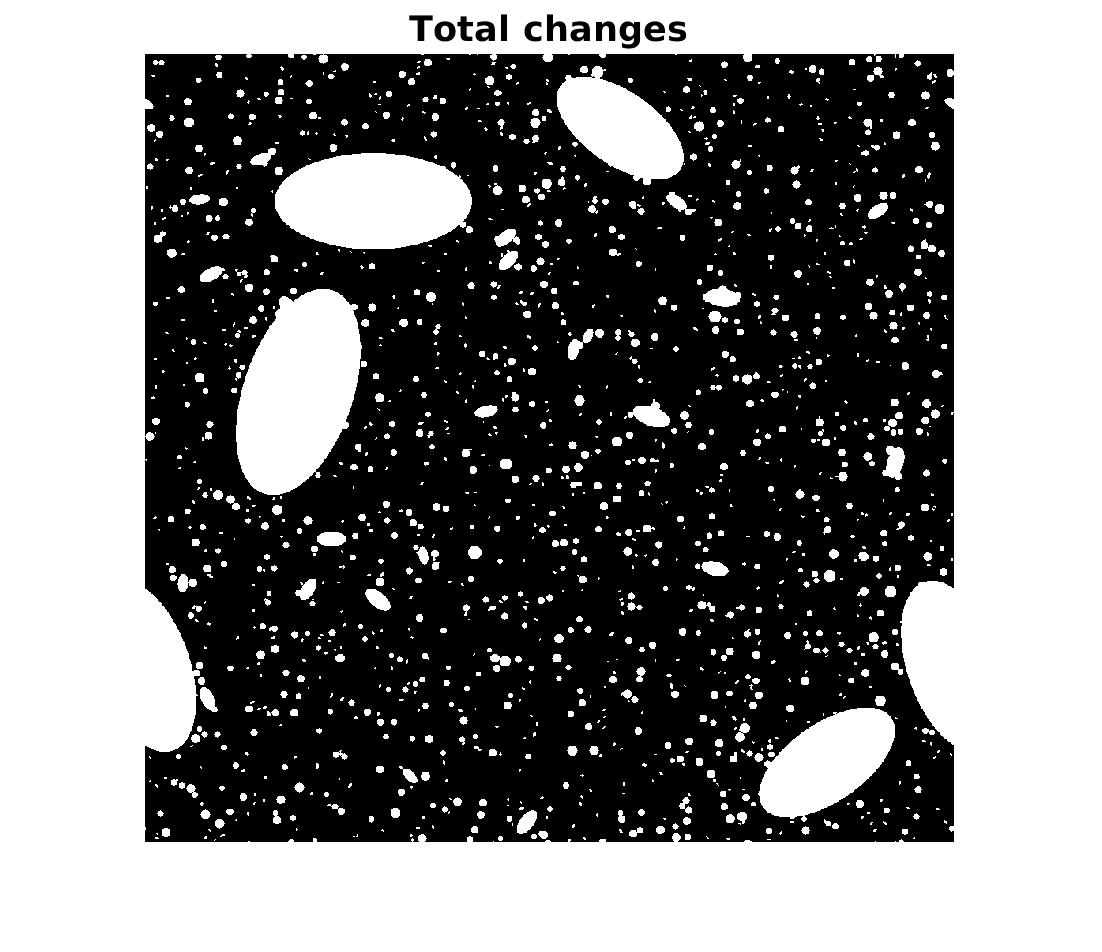
\includegraphics[scale=.1]{../../figs/total_changes}(a)
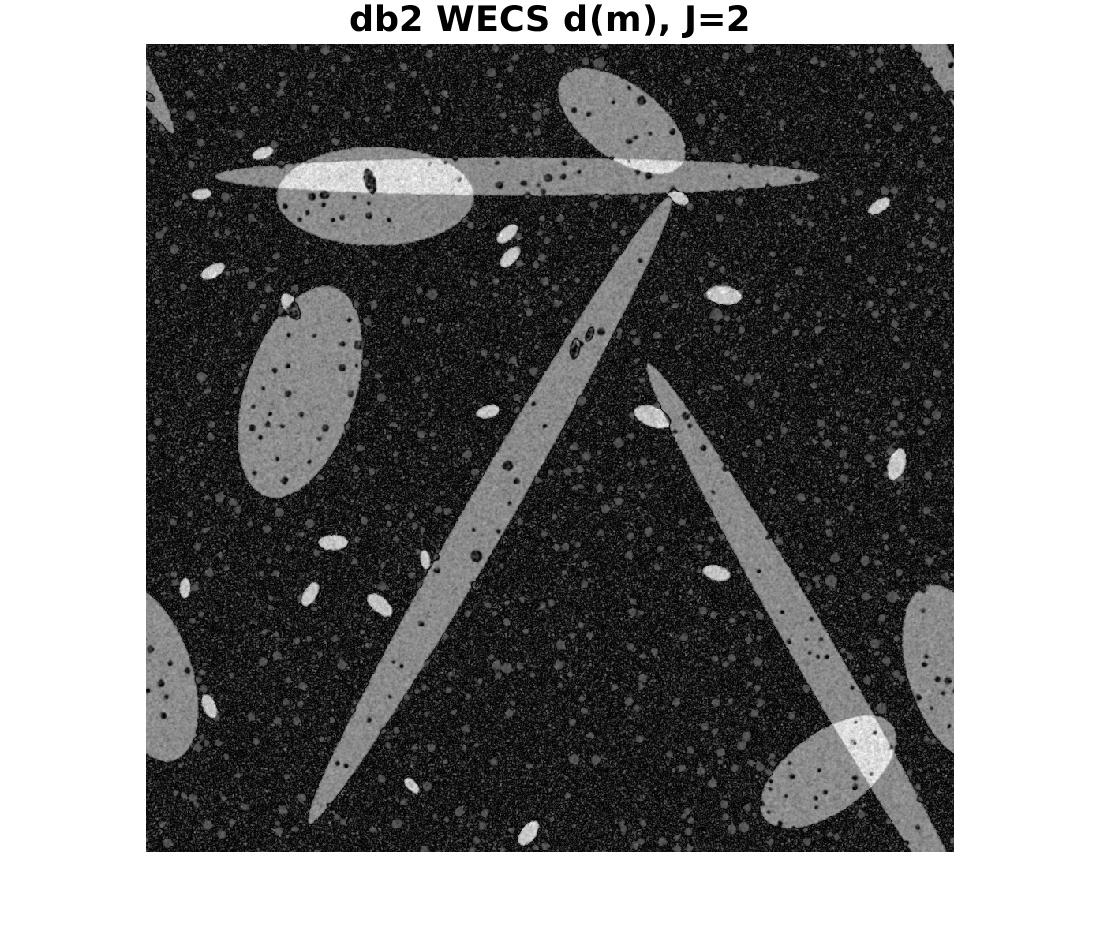
\includegraphics[scale=.1]{../../figs/corr_changes_dm}(b)
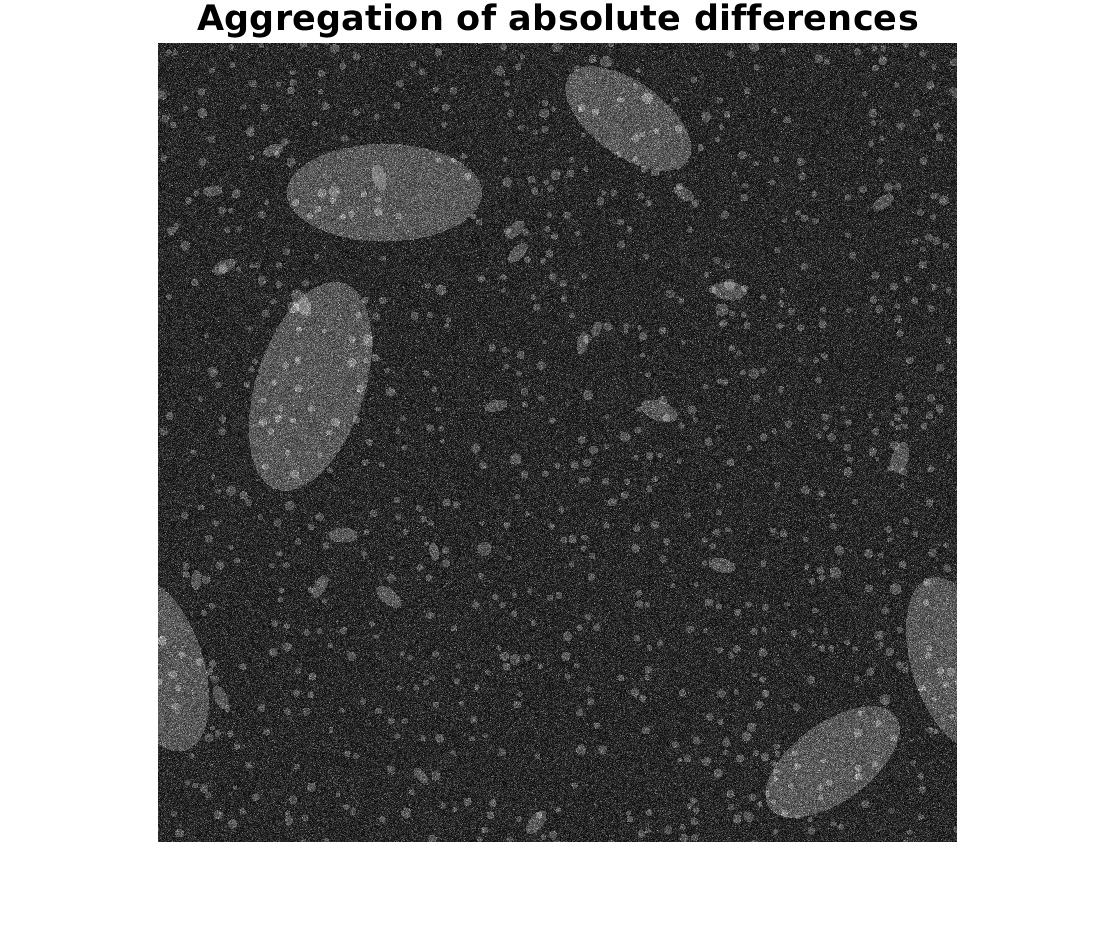
\includegraphics[scale=.1]{../../figs/corr_changes_logratios}(c)
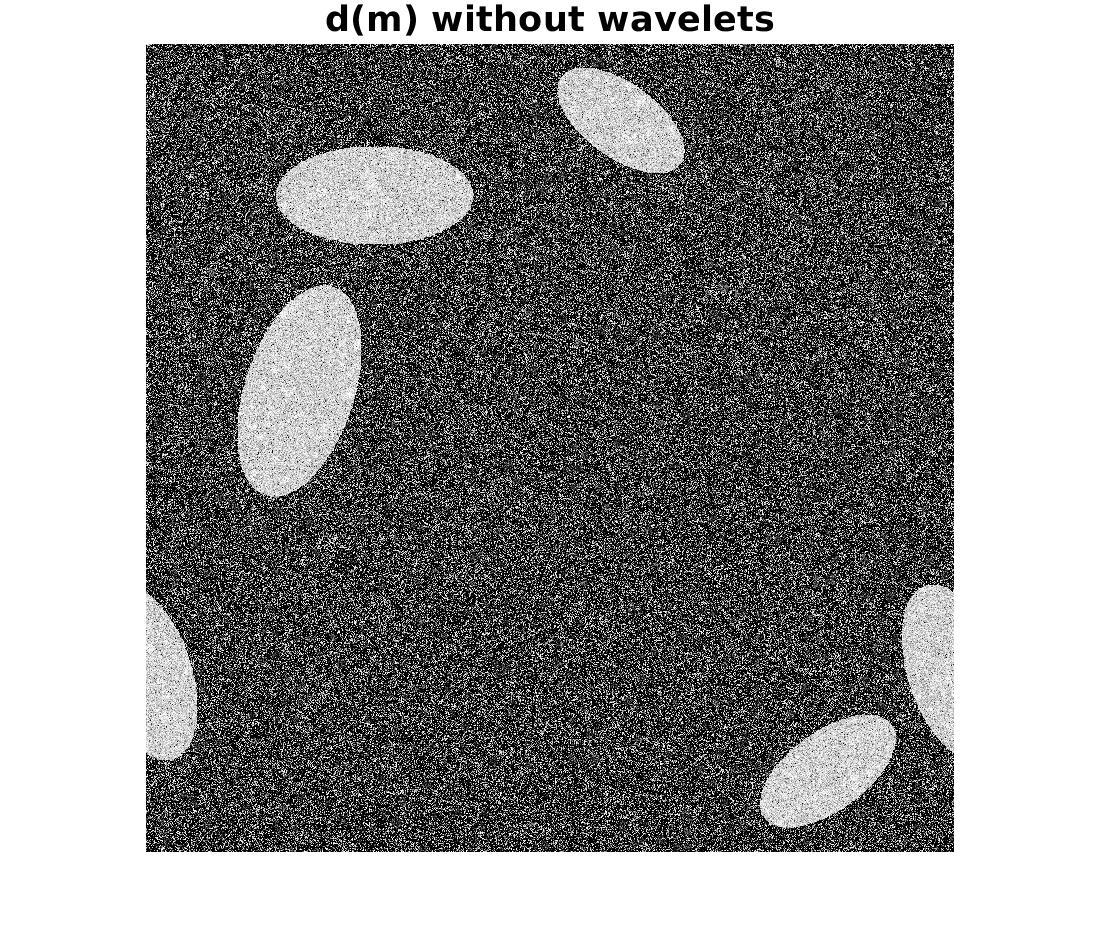
\includegraphics[scale=.1]{../../figs/corr_changes_dm_nowavelets}(d)
\caption{Simulated images with changing ellipses. (a) Image composed by the total changes over time. (b) Proposed db2 WECS $\vd(m)$ with $J=2$; (c) Standard approach. (d) $\vd(m)$ without wavelets.}
\label{F:Changes_methods_images}
\end{figure}

Figure \ref{F:Changes_methods_images} illustrates a comparison of different approaches to detect accumulated changes. Panel (b) shows the result of WECS using Daubechies wavelet with two null moments (db2) and $J=2$. Panel (c) presents the result of using aggregated absolute differences, a standard approach where the accumulation of changes are measured by a matrix $\vS=\{\vS_{k,l}\}$ with $S_{kl} = \sum_{m=2}^n	|\mathcal{I}_{k,l}^{(m)} - \mathcal{I}_{k,l}^{(m-1)}|$. Finally, in Panel (d) we can see the result if $\vd(m)$ is performed purely on the spatial domain, using $\mathcal{I}^{(m)}$ instead of $\vX^{(m)}$ in the WECS formulation. 


We compute ROC curves to compare the detection performance of different methods and to verify the influence of some tuning parameters of wavelet smoothing: the resolution level $J$ and the choice of wavelet basis. Each detection method generates a matrix of change detection measures (correlations in the case of WECS). The ROC curves present the performance of change detection by applying a threshold on these measures, in the following way:
\begin{enumerate}
\item Let $R$ be the matrix of change measures. Compute the range $[r_{\min},r_{\max}]$ of the values in $R$;
\item Let $(r_{(1)},\ldots,r_{(100)})$ be equally space values between $r_{\min}$ and $r_{\max}$;
\item For each $k=1,\ldots,n$, check how many entries are there such that $R_{i,j}>r_{(k)}$ coincide with the element $(i,j)$ where a change really occurs on the image of total changes. Dividing this number by the total number of changes gives the true positive rate.
\item For each $k=1,\ldots,n$, check how many entries are there such that $R_{i,j}>r_{(k)}$  do not coincide with the element $(i,j)$ where a change really occurs. Dividing this number by the total number of entries where changes do not occur gives the false positive rate.
\item The ROC curve is the plot of true and false positive rates corresponding to each $k$.
\end{enumerate}

\begin{figure}[htp!]
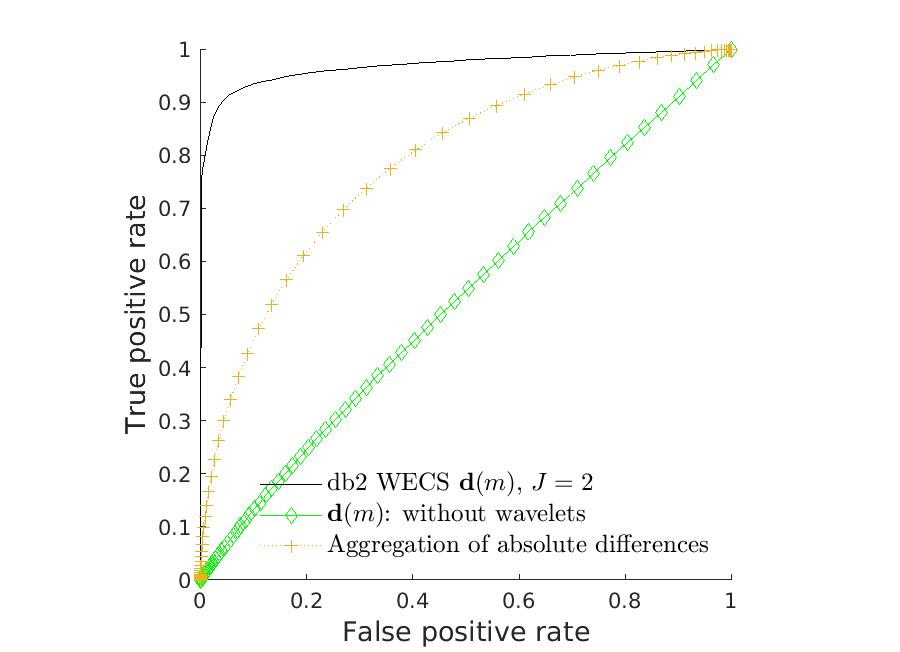
\includegraphics[scale=.13]{../../figs/methods_comparison}\hspace{-.6cm}(a) 
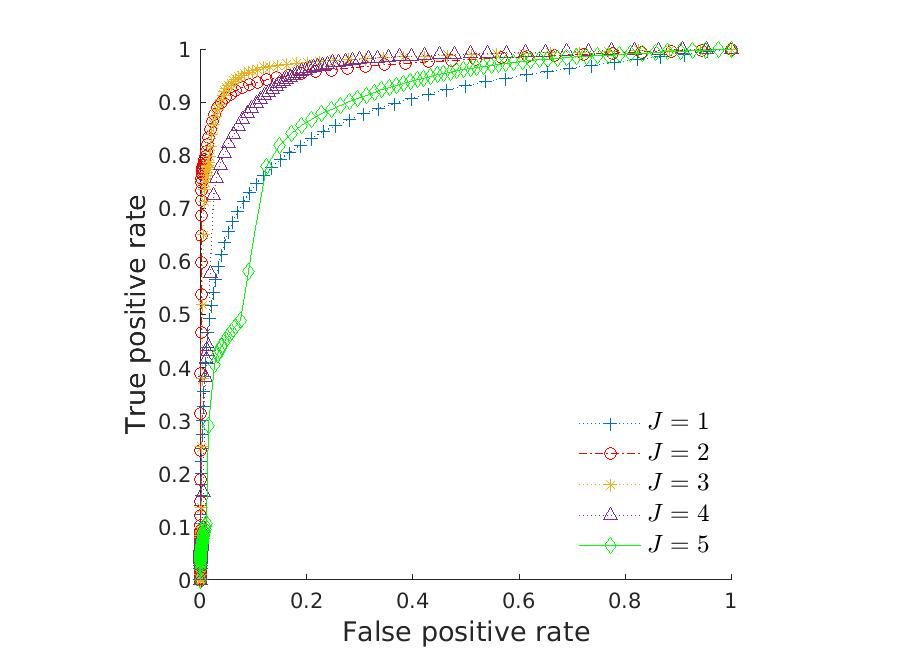
\includegraphics[scale=.13]{../../figs/levels_comparison}\hspace{-.5cm}(b)\\
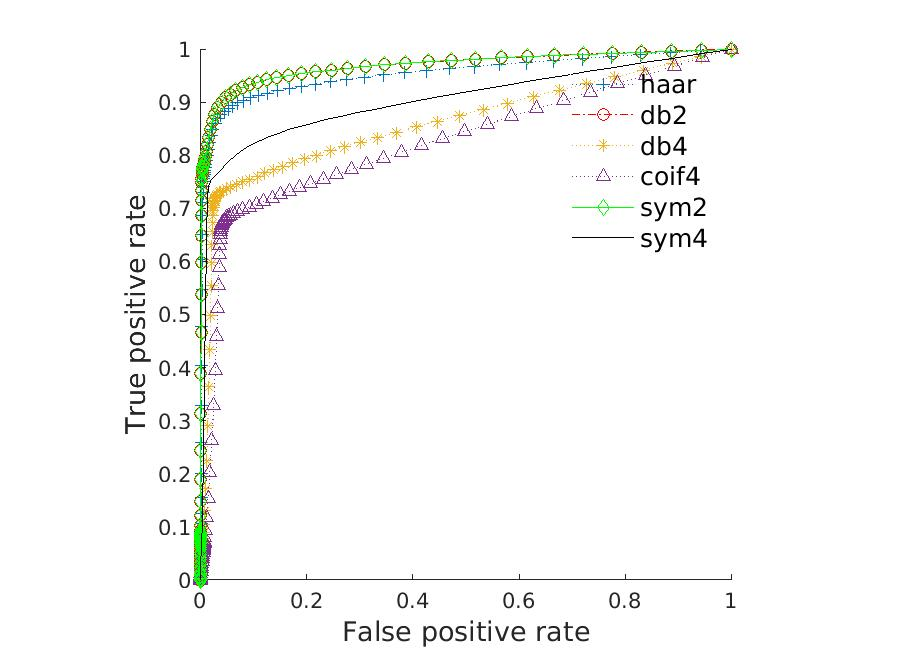
\includegraphics[scale=.13]{../../figs/families_comparison}\hspace{-.5cm}(c)
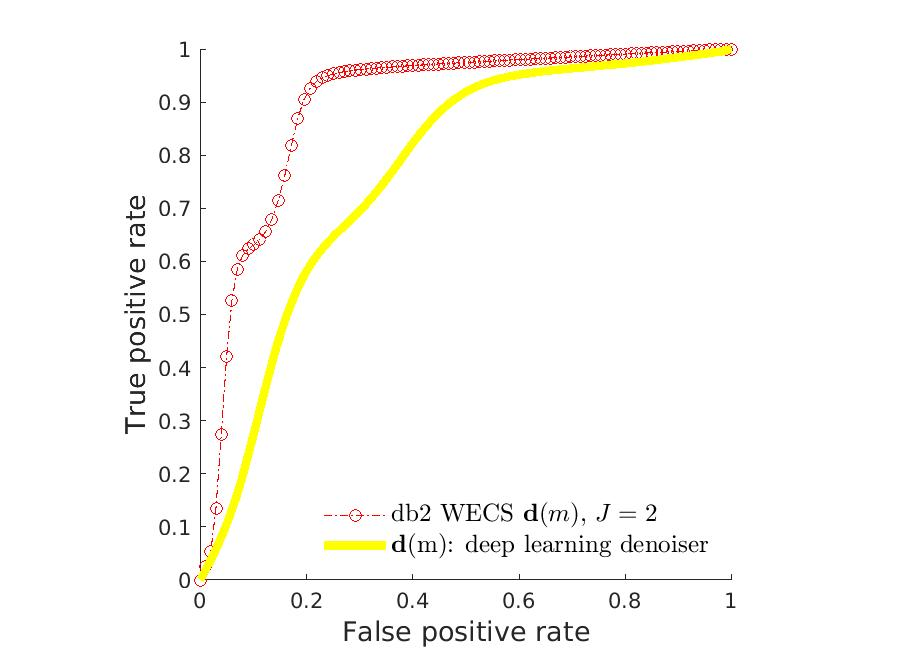
\includegraphics[scale=.13]{../../figs/dm_comparison_wavelet_deepL}\hspace{-.5cm}(d) \\
\caption{ROC curves for detection of changing ellipses in simulated images and different methods. (a) The proposed methods in black (db2 WECS $\vd(m)$) vs two non-wavelet methods: standard log-ratio aggregation (red stars); and $\vd(m)$ (blue).
(b) db2 $\vd(m)$ with different levels.
(c) $\vd(m)$ with different wavelet bases and J=2;
(d) The proposed db2 WECS $\vd(m)$ (red circles) and $\vd(m)$ with deep-learning feature extraction and without wavelets (yellow line).}
\label{F:EllipsoidChanges_details}
\end{figure}

Figure \ref{F:EllipsoidChanges_details} presents the different ROC curves for change detection methods applied to the simulated data as follows. The effects of wavelet bases, level of decomposition, deep-learning feature extraction are shown on the ROC curves. We employ the following wavelet bases: Haar;  Daubechies db2; Daubechies db4; Coiflets coif4; Symlets sym2 ; and Symlets sym4. Panel (c) presents the ROC curves for the proposed method under the aforementioned bases. On all instances $J=2$ is employed. Comparing the ROC curves of all options, we can notice that Daubechies db2 and Symlets sym2 are the best choices.  Panel (b) presents the ROC curves for five different levels of decomposition $J=\{1,2,3,4,5\}$ under the Daubechies db2 basis. Levels $J=2,3$ have a clear better performance, with a slight advantage to $J=2$, since it is uses less levels on the decomposition. The overall performance  of $J=2$ warrants its use for the rest of the comparisons. Panel (d) shows how the proposed method performs in comparison to a deep learning feature extraction from a residual learning network \cite{zhang2017beyond}. WECS is applied with db2 wavelets and $J=2$, whereas the other method applies WECS's idea, the only difference being that $\vX^{(m)}$ is replaced by another smooth version of $\mathcal{I}^{(m)}$ that employs neural-networks trained to compete with wavelet smoothing. We can see that the ROC curves for images treated with a deep-learning method has a performance worse than that obtained with WECS. 
We finally have in Panel (a) the proposed WECS with db2 wavelets and $J=2$ compared to two other non-wavelet methods. The first involves computing $\vd(m)$ without wavelet smoothing, i.e., the squared deviations are computed using $\{\mathcal{I}^{(m)}\}$ instead of $\{\vX^{(m)}\}$, and the classic method of analyzing aggregated absolute differences of $\{\mathcal{I}^{(m)}\}$. The ROC curves in Panel (a) show that the proposed WECS outperforms both the other two methods. 



\subsection{Actual remote sensing application}\label{secExpActual}

We employed the proposed change detection method on a series of 84 multi-date satellite images. The images were taken on a forest region at the border of Brazil and the French Guiana from 2015-12-26 to 2017-12-3. Each image has two channels (VV and VH) and 1538 by 1556 pixels. We perform a change detection wavelet analyses on the combined image by considering each observed entry as $\mathcal{I}_{k,l}^{(m)} = ((\mathrm{VV}_{k,l}^{(m)})^2+(\mathrm{VH}_{k,l}^{(m)})^2)^{1/2}$, where $\mathrm{VV}$ and $\mathrm{VH}$ represent the matrices of observations from VV and VH channels, respectively. 

%-----------------------
\begin{figure}[hbt]
\centering
\includegraphics[width=0.485\textwidth]{../../qgis/maps/StudyArea.pdf}
\caption{Study area location. \textcolor{red}{(preliminar)}}\label{figAE}
\end{figure}


%-----------------------
\begin{figure}[hbt]
\centering

\mbox{
\subfigure[26th December, 2015]{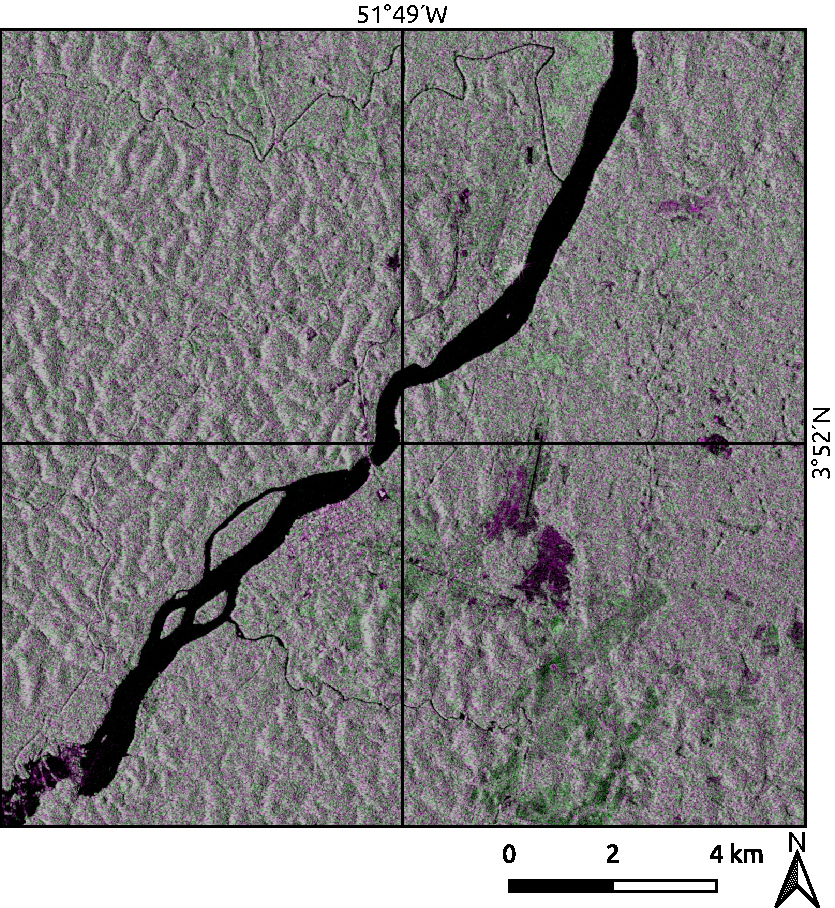
\includegraphics[width=0.23\textwidth]{../../qgis/maps/Sentinel_2015.pdf}\label{figImgSentinel2015}} 
\subfigure[3rd December, 2017]{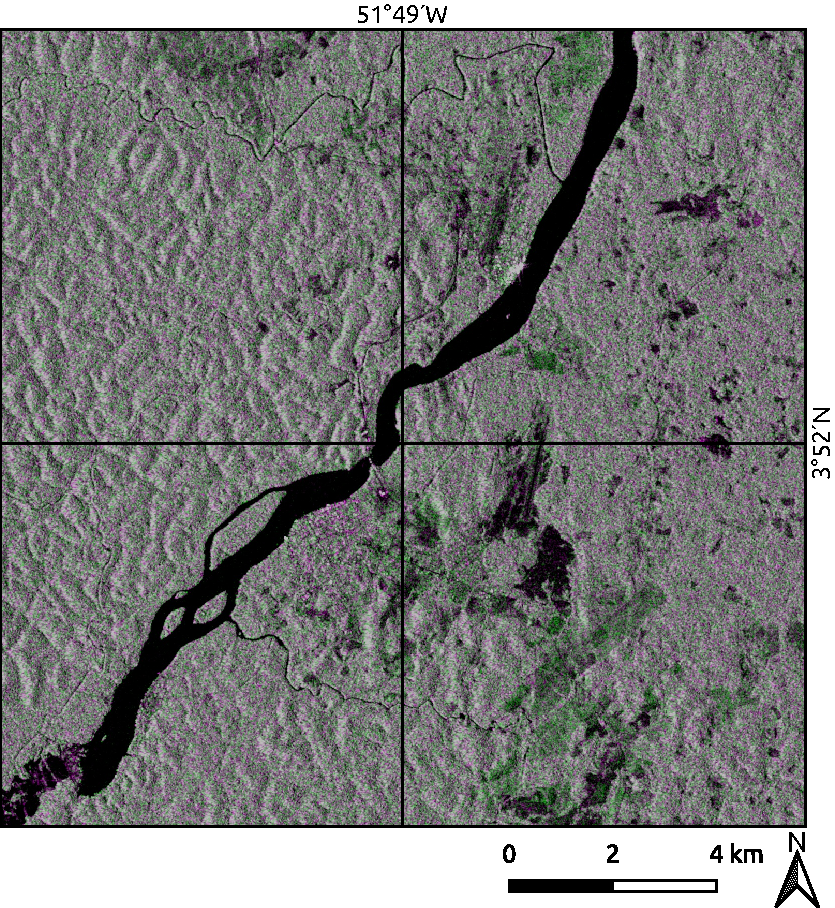
\includegraphics[width=0.23\textwidth]{../../qgis/maps/Sentinel_2017.pdf}\label{figImgSentinel2017}}
}

\subfigure[Ground truth change/non-change samples]{
\includegraphics[width=0.23\textwidth]{../../figs/coming-soon.png}\label{figImgSentinelROIs}}

\caption{\textcolor{red}{Inserir caption...}}\label{figImageRef}
\end{figure}

A multi-resolution analysis based on a Symlet basis with filter of length 16 (symlet 8) is built. In order to have dimensions as power of 2, the matrices $\mathcal{I}_{k,l}$ are extended to a $2048\times2048$ matrix with $\mathcal{I}_{k,l}$ at the center and the remaining parts being completed with mirrored values at the borders. The wavelet transform at resolution level $J=2$ is applied to these matrices and only the portion corresponding to the $1538 \times 1556$ is kept for further processing. Then, we are able to compute the squared mean differences vector $\vd$ and the matrix of absolute correlations $\vR$. 

The time change measures computed with $\vd$ are shown in Figure \ref{F:forest_wecs}. The orange line in Figure \ref{F:forest_wecs}a represents the median absolute deviation of $\vd$, which allow us to notice times that differ expressively from the others. We can notice that times $m=25,27,30$ are highlighted as having the most expressive changes. The images  corresponding to these times can be seen in Figure \ref{F:forest_change_times}.

\begin{figure}[htp!]
\centering
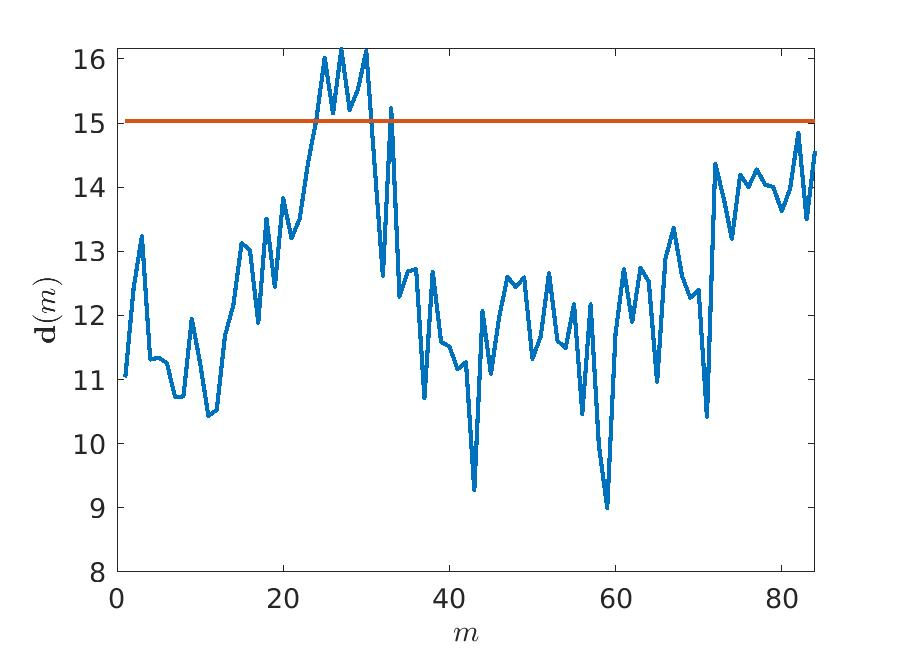
\includegraphics[scale=.2]{../../figs/forest_vSumDifCoefSq}\hspace{-.5cm}
\caption{Plot of $\vd(m)$, $m=1,\ldots,85$ with orange horizontal line indicating two times its median absolute deviation.}
\label{F:forest_wecs}
\end{figure}


\begin{figure}[htp!]
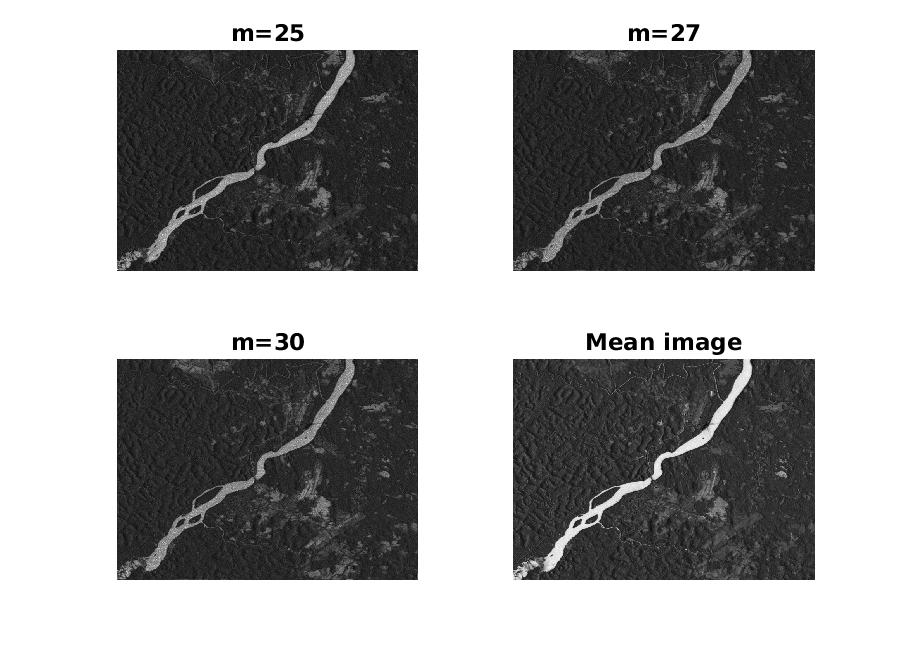
\includegraphics[scale=.3]{../../figs/forest_changes_time} 
\caption{Images $\vX^{(m)}$ from times $m$ correspond to top-3 highest values of $\vd(m)$ and the mean image $\bar{\mathcal{I}}$.}
\label{F:forest_change_times}
\end{figure}

The changes in space can be analyzed using the image obtained with $\vR$, which is displayed in Figure \ref{F:forest_wecs}c. Denoting the images' dimension as $N=1538\times1556$, if we take the $[N/\log N]$ largest absolute correlations as those corresponding to possible change points, we obtain a matrix of zeros and ones that is presented in Figure \ref{F:forest_wecs}e. The white regions in Figure \ref{F:forest_wecs}c (entries with value one) represent the change points, which seem to concentrate mainly on three regions: at the center, to the right of the river; at the top, on the left border of the river; and at the top left. Computing aggregated absolute differences to measure changes in space, we obtain Figure \ref{F:forest_wecs}d. An image of detected changes corresponding to measures in  Figure \ref{F:forest_wecs}d can be obtained applying a thresholding method for grayscale images.  Figure \ref{F:forest_wecs}f shows the result of using Otsu's thresholding method \cite{otsu1979threshold} for aggregation of absolute differences.

The comparison of performance for the two change detection measures considered here can be checked in Figure \ref{F:forest_roc_wecs_agg}, where a ROC curve is computed to check the correct detection of changes. WECS attains high true positive rates before the aggregation method, but both methods design competitive results. This performance differs from the ROC curve results in the previous section because the real images have a mean signal to noise ratio (SNR) of 3.9327, whereas the simulated images were generated with SNR of 0.2309. Hence, WECS is expected to have performance closer to the aggregation method in less noisy applications. The reference of correct change regions is shown in Figure \ref{F:forest_roc_wecs_agg}a, which are determined using [XXXXX]. 

We can also compare the change detection methods using the $F_1$-score accuracy measure. Denoting $\mathrm{TP}$ as the number of true positives (change pixels correctly detected), $\mathrm{FP}$ as the number of false positives (nonchange pixels flagged as change point) and $\mathrm{FN}$ as the total of false negatives (change points flagged as nonchange point), the $F_1$-score is defined as
\begin{equation*}
F_1 = 2\frac{\mathrm{Pr}\cdot\mathrm{Re}}{\mathrm{Pr}+\mathrm{Re}}	,
\end{equation*}
where
\begin{equation*}
\mathrm{Pr}=\frac{\mathrm{TP}}{\mathrm{TP}+\mathrm{FP}}\quad 
\text{and} \quad \mathrm{Re} = \frac{\mathrm{TP}}{\mathrm{TP}+\mathrm{FN}}.
\end{equation*}
Results of these three accuracy measures are presented in Table \ref{T:forest_accuracy}. Results for aggregation of absolutes differences correspond to two types of thresholds: Otsu's method and Kittler-Illingworth \cite{kittler1986minimum}. We can observe that WECS presents the highest value of $F_1$-score, which means it has a better performance that the competing method.

\begin{figure}[htp!]
\centering
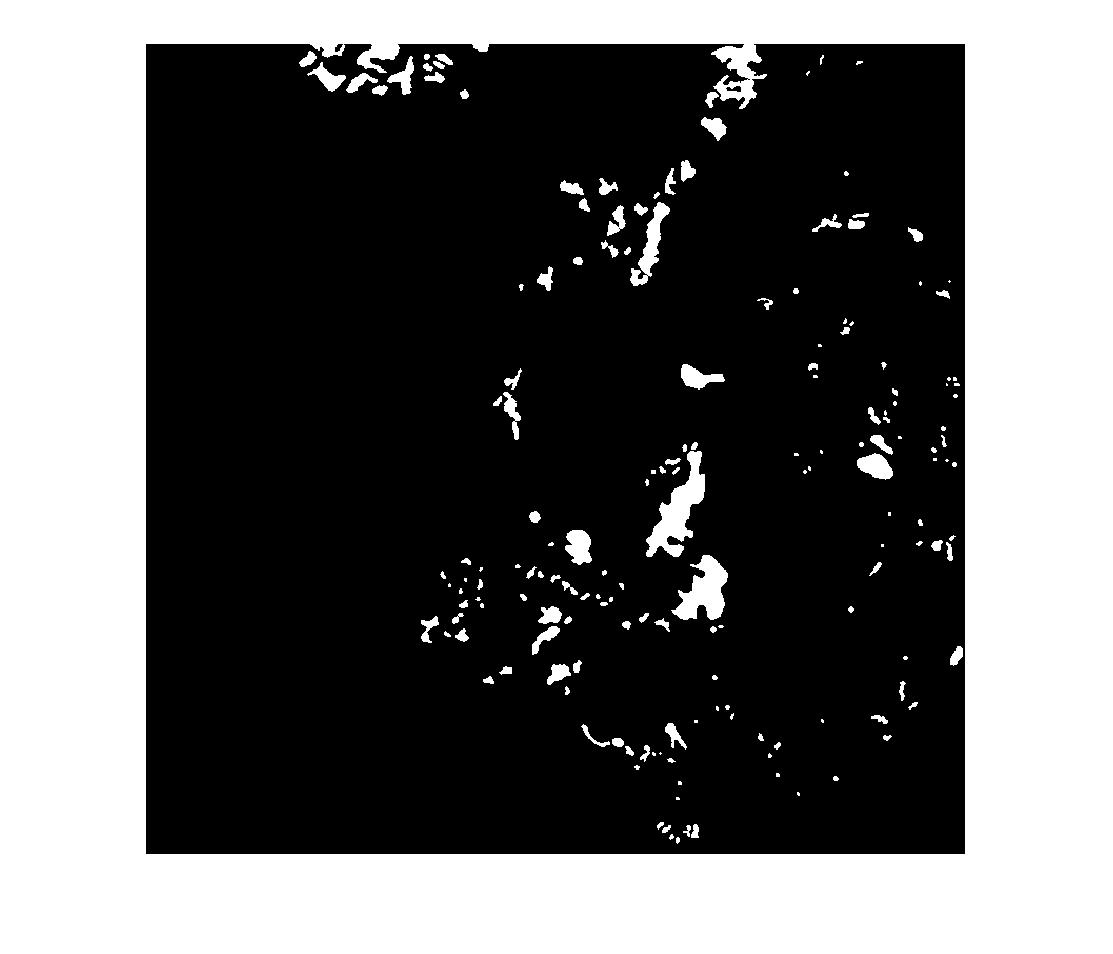
\includegraphics[scale=.10]{../../figs/forest_change}\hspace{-.5cm}(a)
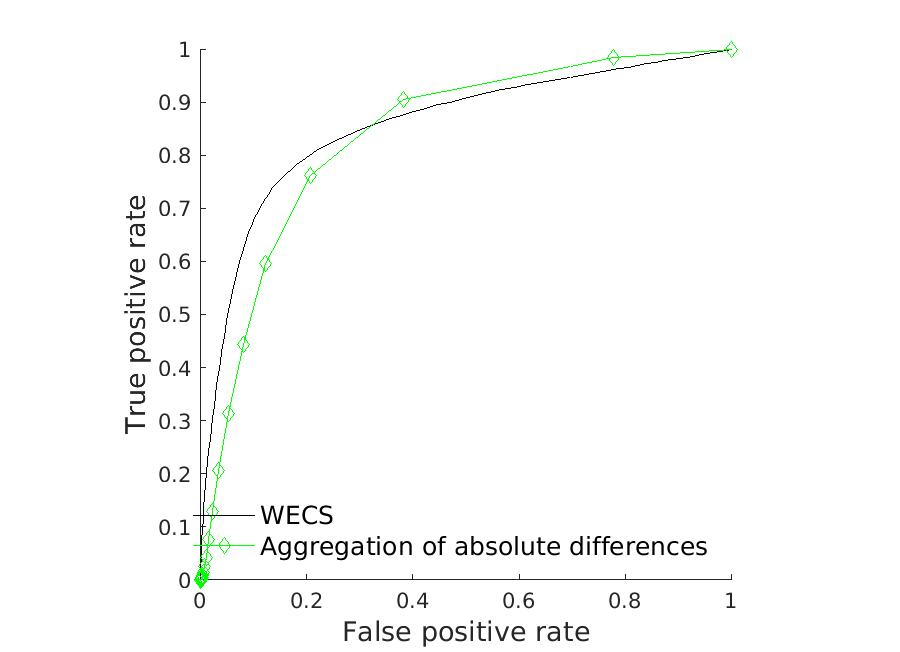
\includegraphics[scale=.15]{../../figs/forest_roc_change}\hspace{-.5cm}(b)\\
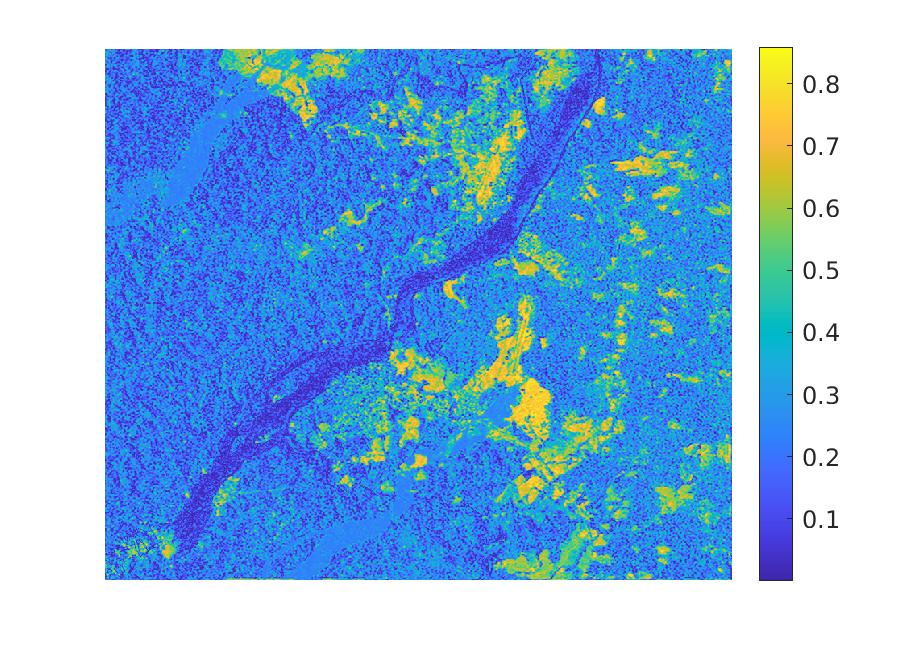
\includegraphics[scale=.13]{../../figs/forest_wecs_abscorr}\hspace{-.5cm}(c)
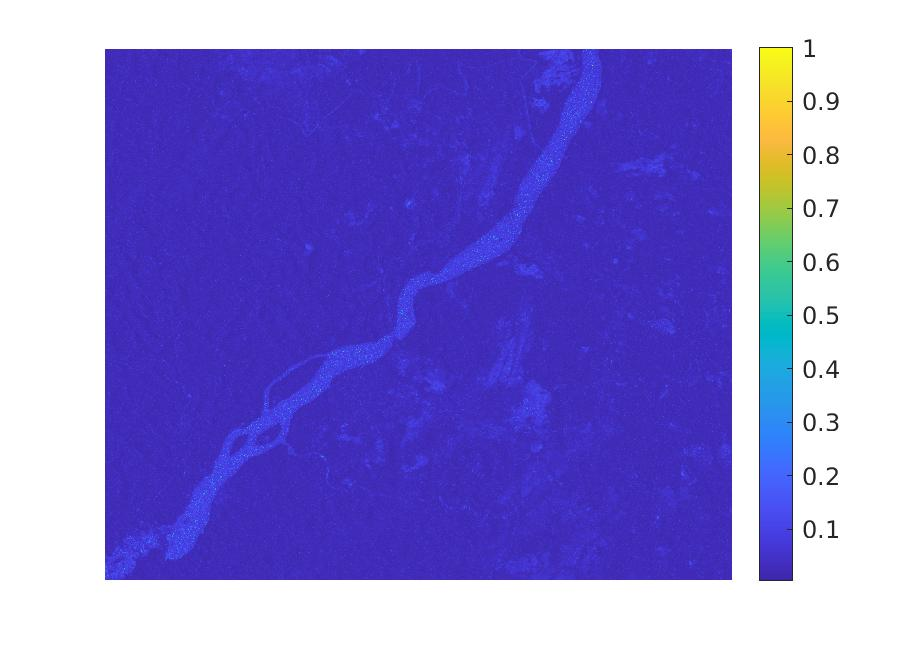
\includegraphics[scale=.13]{../../figs/forest_aggreg_ratios}\hspace{-.5cm}(d)\\
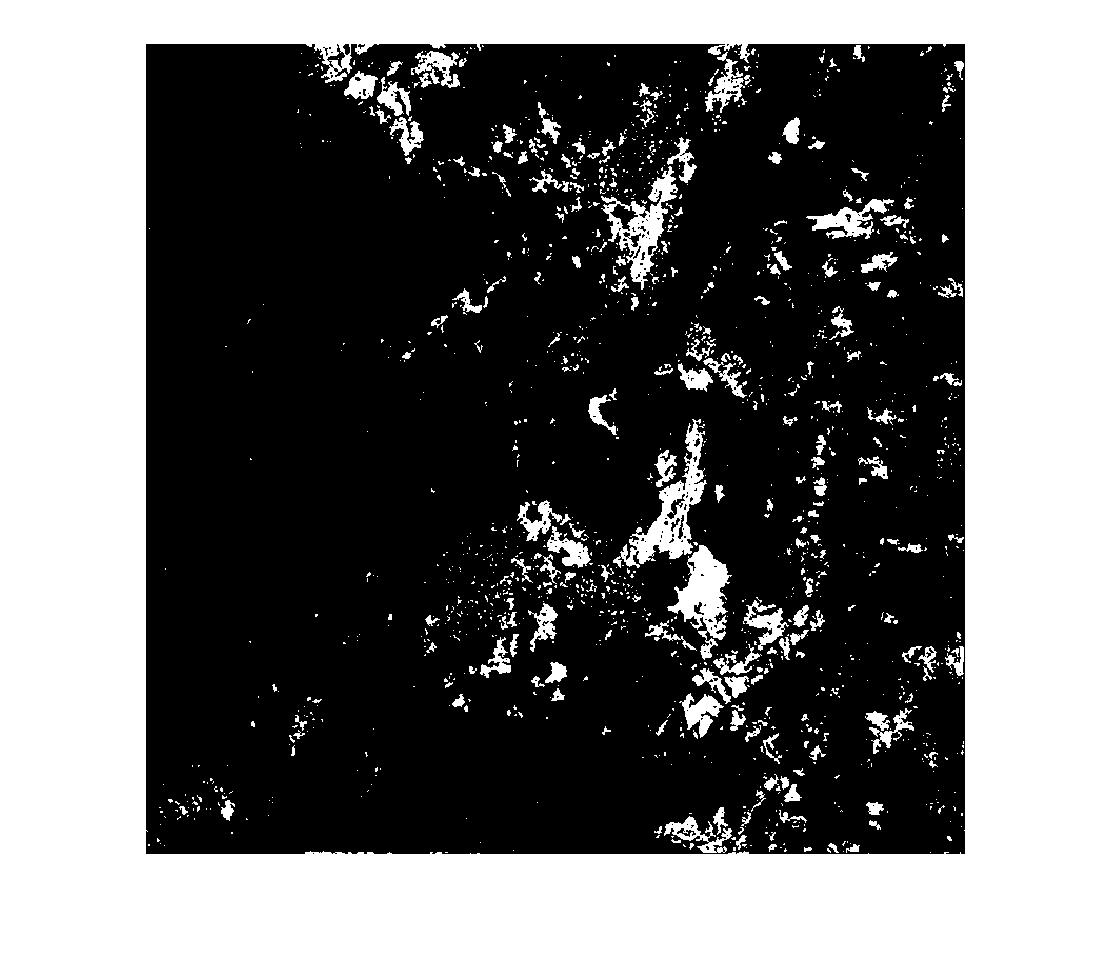
\includegraphics[scale=.10]{../../figs/forest_wecs_change_space}\hspace{-.5cm}(e) 
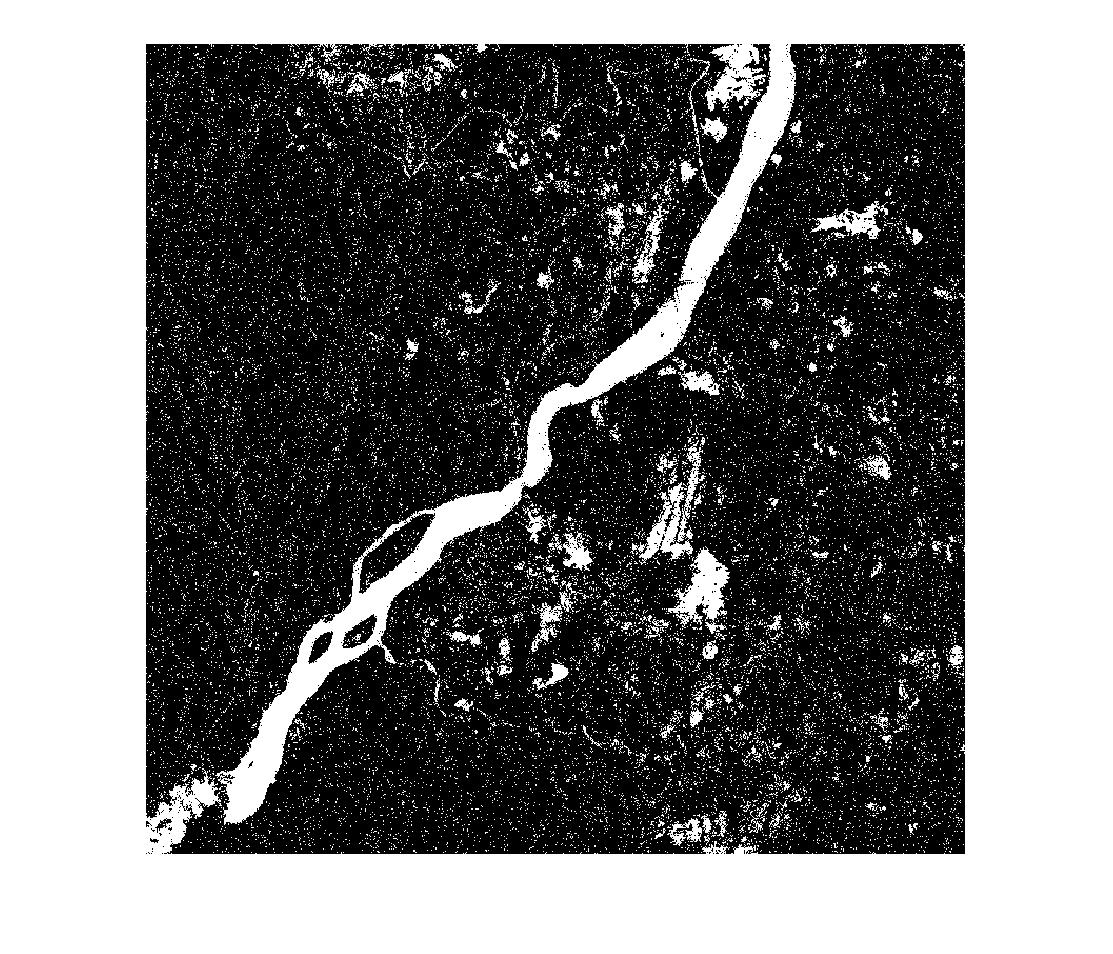
\includegraphics[scale=.10]{../../figs/forest_aggreg_change_space}\hspace{-.5cm}(f)\\ 
\caption{Change points in space of the forest data. (a) Regions (in white) where changes should be detected. (b) ROC curve for detection of changing regions. (c) Matrix of absolute correlations obtained with WECS. (d) Change measures from aggregation of absolute differences. (e) Change regions detected by highlighting the $[N/\log N]$ largest correlations in $\vR$ ($N$ denoting the image's dimension). (f) Change regions detected using aggregated absolute differences and Otsu's thresholding.}
\label{F:forest_roc_wecs_agg}
\end{figure}


\begin{table}
\caption{Accuracy measures $F_1$-score, Precision ($\mathrm{Pr}$) and Recall ($\mathrm{Re}$) computed from detection of changing regions in the forest data using WECS (taking the $[N/\log N]$ largest correlations as corresponding to change) and the aggregation of absolute differences with Otsu and Kittler-Illingworth's (KI) thresholds.}
\centering
\begin{tabular}{c|ccc}
\hline
  & Aggregated - Otsu & Aggregated - KI & WECS \\
\hline
$F_1$-score & 0.2231 & 0.2163 & 0.3253 \\
$\mathrm{Pr}$ & 0.1369 & 0.1296 & 0.2390 \\
$\mathrm{Re}$ & 0.6022 & 0.6526 & 0.5094 \\
\hline
\end{tabular}
\label{T:forest_accuracy}
\end{table}


\section{Discussion}\label{section_discussion}

We present a novel way of detecting changes in multi-temporal satellite images, WECS. The procedure is based on wavelet energies from both the estimated individual coefficients as well as the whole mean image. It makes use of correlation screening for ultra-high dimensional data. Thereupon, WECS is expected to provide a sample of points in space in a way that such set, contains real change points with high probability. The proposed method's performance is shown using both simulated and real data. The proposed method is useful to detect spatio-temporal change points, which is illustrated on data analyses. The method is employed to analyze a time series of 84 images of a forest.




% if have a single appendix:
%\appendix[Proof of the Zonklar Equations]
% or
%\appendix  % for no appendix heading
% do not use \section anymore after \appendix, only \section*
% is possibly needed

% use appendices with more than one appendix
% then use \section to start each appendix
% you must declare a \section before using any
% \subsection or using \label (\appendices by itself
% starts a section numbered zero.)
%

%
%\appendices
%\section{Proof of the First Zonklar Equation}
%Appendix one text goes here.

% you can choose not to have a title for an appendix
% if you want by leaving the argument blank
%\section{}
%Appendix two text goes here.


% use section* for acknowledgment
%\section*{Acknowledgment}



% Can use something like this to put references on a page
% by themselves when using endfloat and the captionsoff option.
\ifCLASSOPTIONcaptionsoff
  \newpage
\fi



% trigger a \newpage just before the given reference
% number - used to balance the columns on the last page
% adjust value as needed - may need to be readjusted if
% the document is modified later
%\IEEEtriggeratref{8}
% The "triggered" command can be changed if desired:
%\IEEEtriggercmd{\enlargethispage{-5in}}

% references section

% can use a bibliography generated by BibTeX as a .bbl file
% BibTeX documentation can be easily obtained at:
% http://mirror.ctan.org/biblio/bibtex/contrib/doc/
% The IEEEtran BibTeX style support page is at:
% http://www.michaelshell.org/tex/ieeetran/bibtex/
\bibliographystyle{IEEEtran}
% argument is your BibTeX string definitions and bibliography database(s)
\bibliography{bibfile}
%
%% <OR> manually copy in the resultant .bbl file
%% set second argument of \begin to the number of references
%% (used to reserve space for the reference number labels box)
%\begin{thebibliography}{1}
%
%\bibitem{IEEEhowto:kopka}
%H.~Kopka and P.~W. Daly, \emph{A Guide to \LaTeX}, 3rd~ed.\hskip 1em plus
%  0.5em minus 0.4em\relax Harlow, England: Addison-Wesley, 1999.
%
%\end{thebibliography}

% biography section
% 
% If you have an EPS/PDF photo (graphicx package needed) extra braces are
% needed around the contents of the optional argument to biography to prevent
% the LaTeX parser from getting confused when it sees the complicated
% \includegraphics command within an optional argument. (You could create
% your own custom macro containing the \includegraphics command to make things
% simpler here.)
%\begin{IEEEbiography}[{\includegraphics[width=1in,height=1.25in,clip,keepaspectratio]{mshell}}]{Michael Shell}
% or if you just want to reserve a space for a photo:


%\begin{IEEEbiography}
%[{\includegraphics[width=1in,height=1.25in,clip,keepaspectratio]{../Photo/rodney}}]{Rodney Fonseca}
%was born in Brazil, in 1993. He received the Master’s
%degrees in Statistics from the Federal University of Pernambuco,
%Recife, Brazil, in 2017, and the Ph.D. degree in Statistics, from Campinas State University, Campinas, Brazil, in 2021.
%His research interests include nonparametric statistics, time series, graph signal processing and regression models.
%\end{IEEEbiography}
%\vfill
%
%\begin{IEEEbiography}[{\includegraphics[width=1in,height=1.25in,clip,keepaspectratio]{../Photo/aluisio}}]{Alu\'{i}sio~Pinheiro}
%was born in Brazil, in 1967. He received the Master’s degree in Statistics from Campinas State University, Campinas, Brazil, in 1992, and the Ph.D. degree in Statistics from University of North Carolina, Chapel Hill, US, in 1997.
%He is currently Professor at Campinas State University. His research interests concern U-statistics, wavelets, nonparametric statistics and time series.
%Dr. Pinheiro was the 2012 Pranab Kumar Sen Distinguished Visiting Professor of Biostatistics, UNC-Chapel Hill. He has been the Brazilian Statistics Association General Secretary (2010-2012) and Treasurer (2018-2020).
%\end{IEEEbiography}
%
%
%\begin{IEEEbiography}[{\includegraphics[width=1in,height=1.25in,clip,keepaspectratio]{../Photo/abdou}}]{Abdourrahmane Mahamane Atto}
%was born in Niger, in 1974. He received the Master’s
%degrees in applied mathematics and pure mathematics from the University of Abomey-Calavi,
%Cotonou, Benin, 2001 and 2002, respectively, the
%Master’s degree of advanced studies in electrical engineering from the École Polytechnique d’Abomey-Calavi, Cotonou, in 2002, and the Ph.D. degree
%in applied mathematics, codelivered by TELECOM
%Bretagne, Brest, France, and the University of
%Rennes I, Rennes, France, in 2008.
%He worked with École Polytechnique d’Abomey-Calavi, from 2002 to 2003,
%Ecole des Mines, de l’Industrie et de la Géologie, Niamey, Niger, from 2003
%to 2004, TELECOM Bretagne, from 2008 to 2009, and Institut Polytechnique
%de Bordeaux, Talence, France, from 2009 to 2011. Since September 2011, he
%has been an Associate Professor at the University of Savoie, Polytech Annecy-Chambéry, Annecy, France. His research interests concern mathematical methods and models for signal, image, and information processing.
%\end{IEEEbiography}
%\vfill

% You can push biographies down or up by placing
% a \vfill before or after them. The appropriate
% use of \vfill depends on what kind of text is
% on the last page and whether or not the columns
% are being equalized.

%\vfill

% Can be used to pull up biographies so that the bottom of the last one
% is flush with the other column.
%\enlargethispage{-5in}



% that's all folks
\end{document}


